\chapter{Gravimetrie}


Das Ziel einer gravimetrischen Messung ist die Untersuchung des Untergrunds auf Anomalien der Dichte, um die Massenverteilung rekonstruieren zu können. Damit lassen sich beispielsweise Unterschiede im Gestein lokalisieren. \par

 Hierzu vermisst man das lokale Schwerefeld der Erde, das durch Dichteunterschiede im Boden geringfügig verändert wird. Um diese Änderungen messen zu können, werden hoch empfindliche Messgeräte verwendet.\par
 
 Im Folgenden werden wir uns mit zugrunde liegenden physikalischen Prinzipien, sowie den Störfaktoren und deren Korrektur beschäftigen. Weiterhin wird es einen kurzen Einblick in die Messmethodik geben.

\section{Physikalische Grundlagen}


\subsection*{Gravitationsgesetz}
Die Anziehung zweier punktförmiger Massen wird durch das Newton'sche Gravitationsgesetz beschrieben. Hierbei bezeichnet $|\vec{F}|$ den Betrag der vektoriellen Kraft, $m_1$ und $m_2$ die betrachteten Massen, $r$ den Abstand der Massenmittelpunkte und $G$ die Gravitationskonstante. Letztere ist eine universelle Größe und gilt in allen Bezugssystemen. 

\begin{equation*}
	|\vec{F}| = G \frac{m_1 \cdot m_2}{r^2} \quad \text{mit}\quad G = 6,67 \cdot 10^{-11}\,\frac{\si{m^3}}{\si{kg s^2}}
\end{equation*} 

\begin{figure}[H]
  \centering
  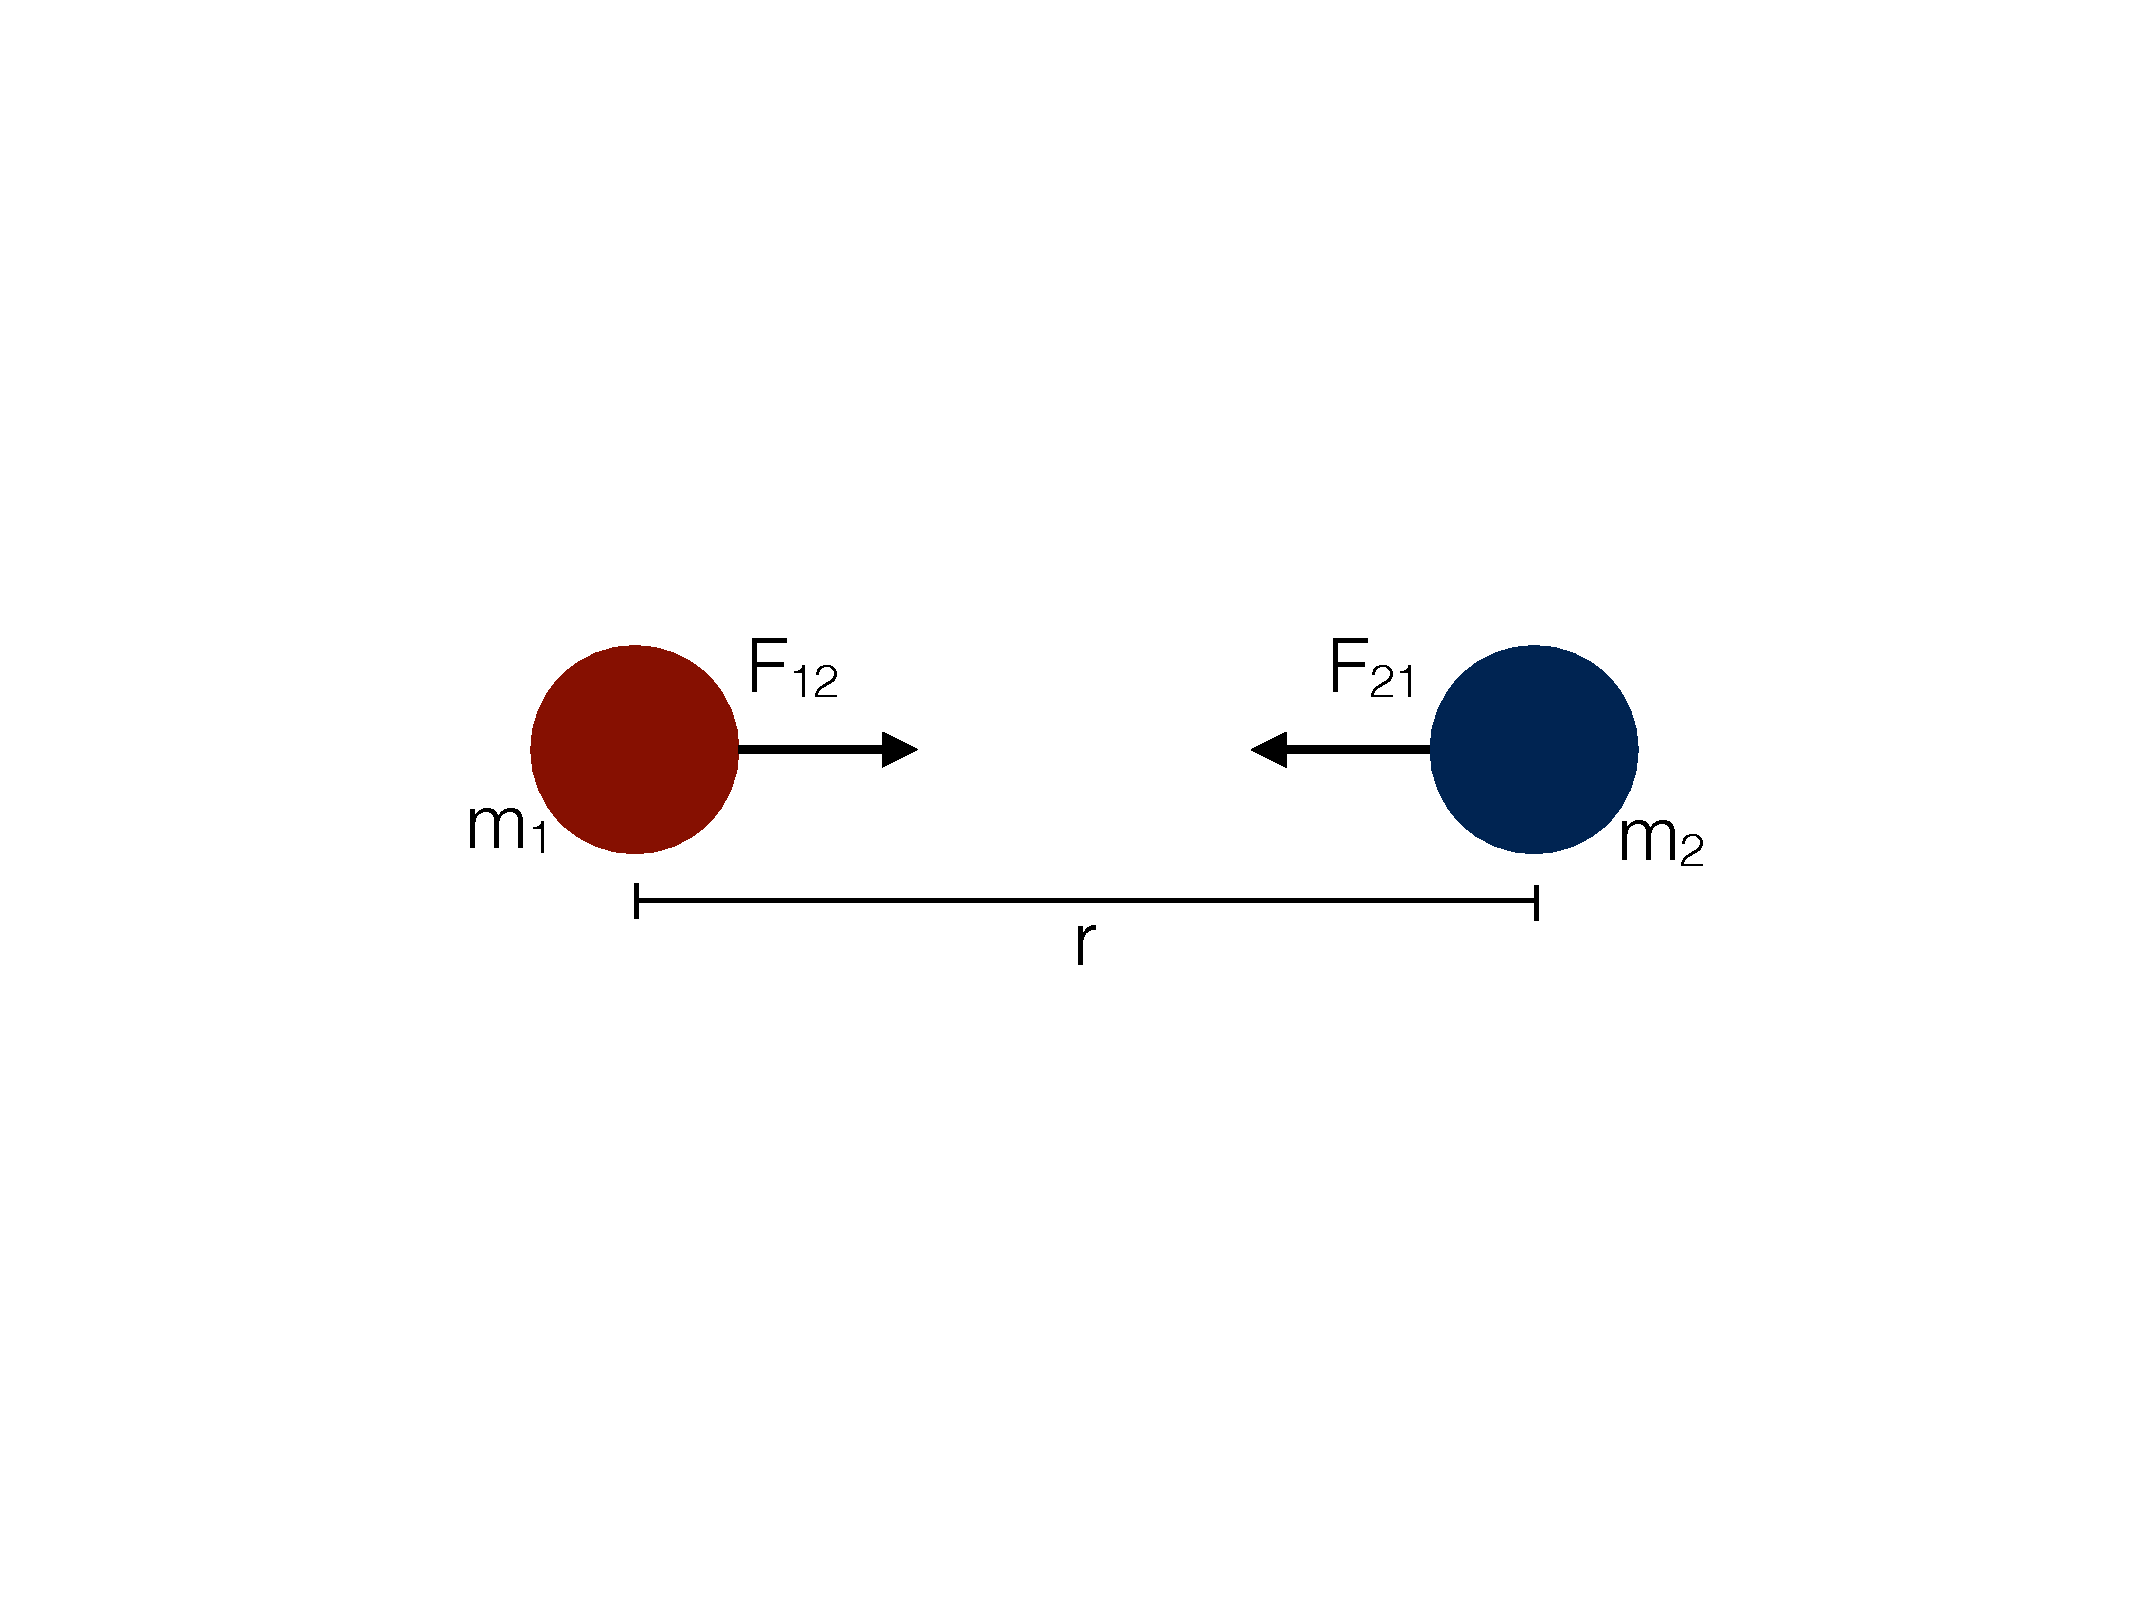
\includegraphics[width = \textwidth]{GravimetrieBilder/GravitationGrafik}
\end{figure}

\section{Das Schwerefeld und die Figur der Erde}

Betrachten wir nun das Gravitationsgesetz im Bezug zur Erde. Dabei gehen wir von einer Kugelerde mit Radius $R = 6371\,\si{km} $ aus.\\
Wir bezeichnen die Masse der Erde für den Rest dieses Kapitels mit $M$ und eine beliebige Masse an der Erdoberfläche mit $m$. In der folgenden Formel berechnen wir die Erdanziehungskraft eines Objekts mit Masse $m$: 


\begin{figure}[H]
	\begin{subfigure}[m]{0.5\textwidth}
	\centering
		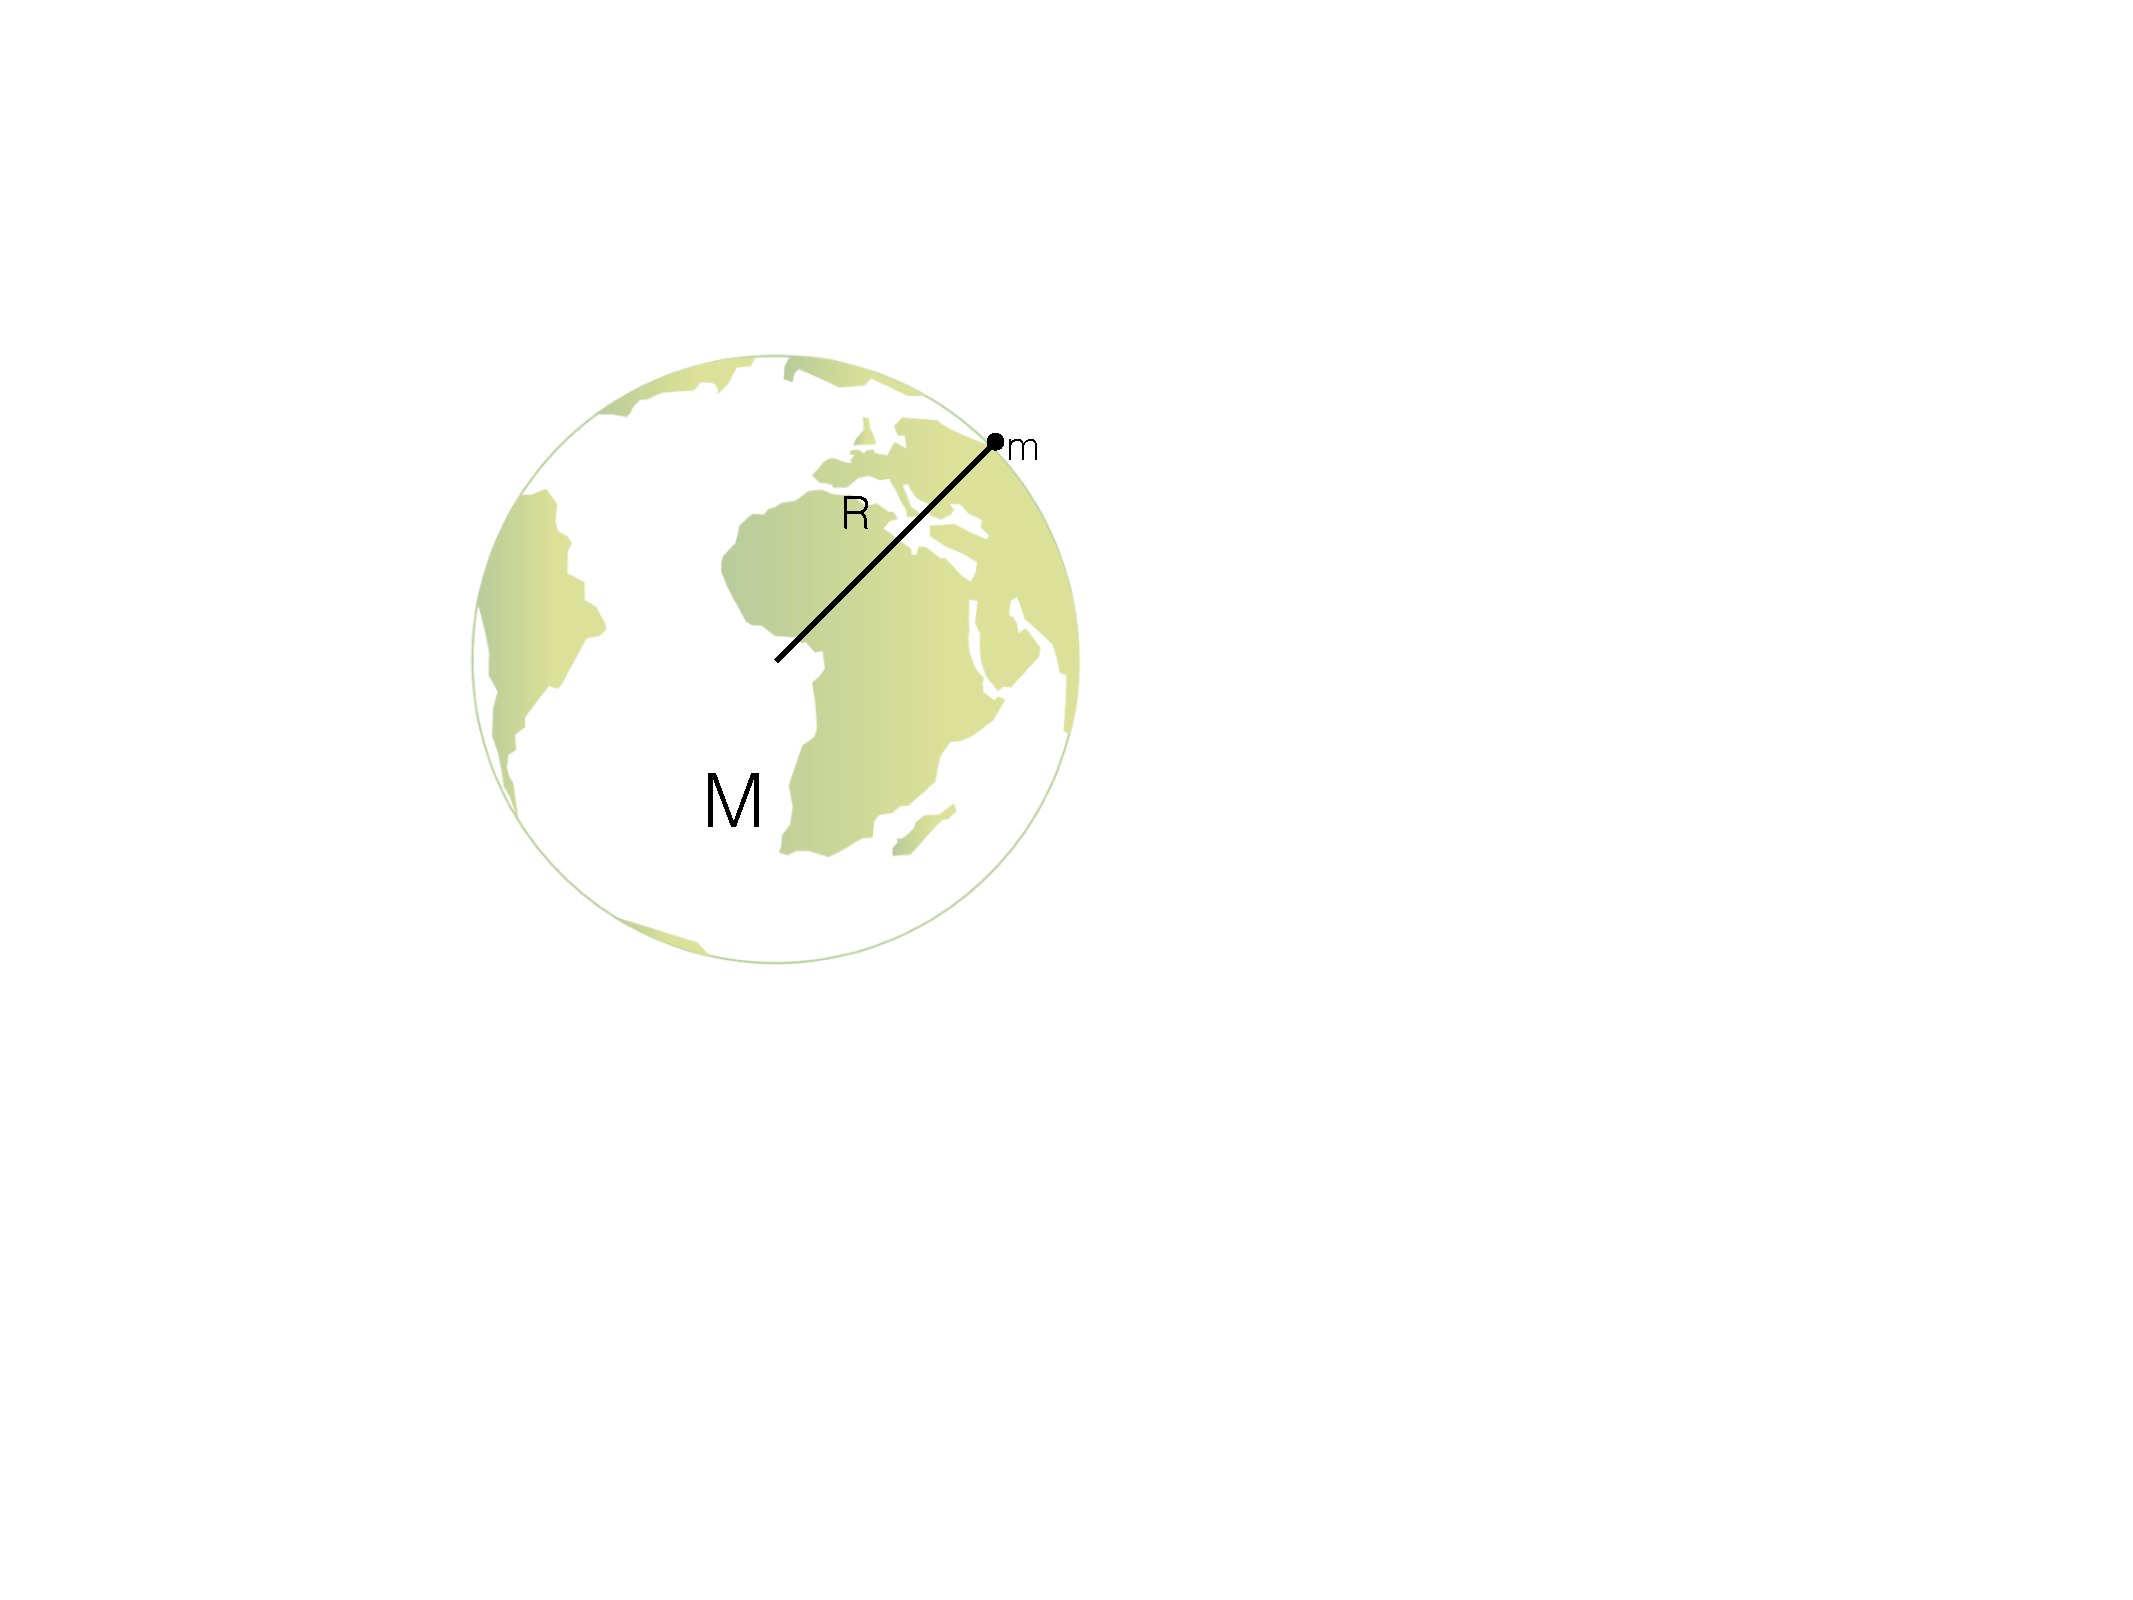
\includegraphics[scale=0.3]{GravimetrieBilder/Erde_mit_Masse_und_Radius}
	\end{subfigure}
	\begin{subfigure}[m]{0.5\textwidth}
	\centering
		\[\begin{aligned}
			|\vec{F}| = \frac{G\cdot M}{R^2} \cdot m = g_0 \cdot m
		\end{aligned}\]
	\end{subfigure}
\end{figure}


$g_0$ ist die Normalbeschleunigung, also die mittlere Fallbeschleunigung auf der Erdoberfläche:

\begin{equation*}
	g_0 = 9,81\,\frac{\si{m}}{\si{s^2}} = 981\,\frac{\si{cm}}{\si{s^2}} = 981\,\si{Gal}
\end{equation*} 

Die nachfolgende Grafik stellt die Schwerebeschleunigung in Abhängigkeit vom Abstand vom Erdmittelpunkt dar. Wir beobachten, dass im Erdmittelpunkt \mbox{$g=0$} gilt und die Schwerebeschleunigung danach bis zu ihrem Maximum $g_0$ bei $R$ linear zunimmt. Für Abstände größer als den Erdradius nimmt sie proportional zu $1/r^2$ ab und geht gegen Null. 

\begin{figure}[H]
\centering
  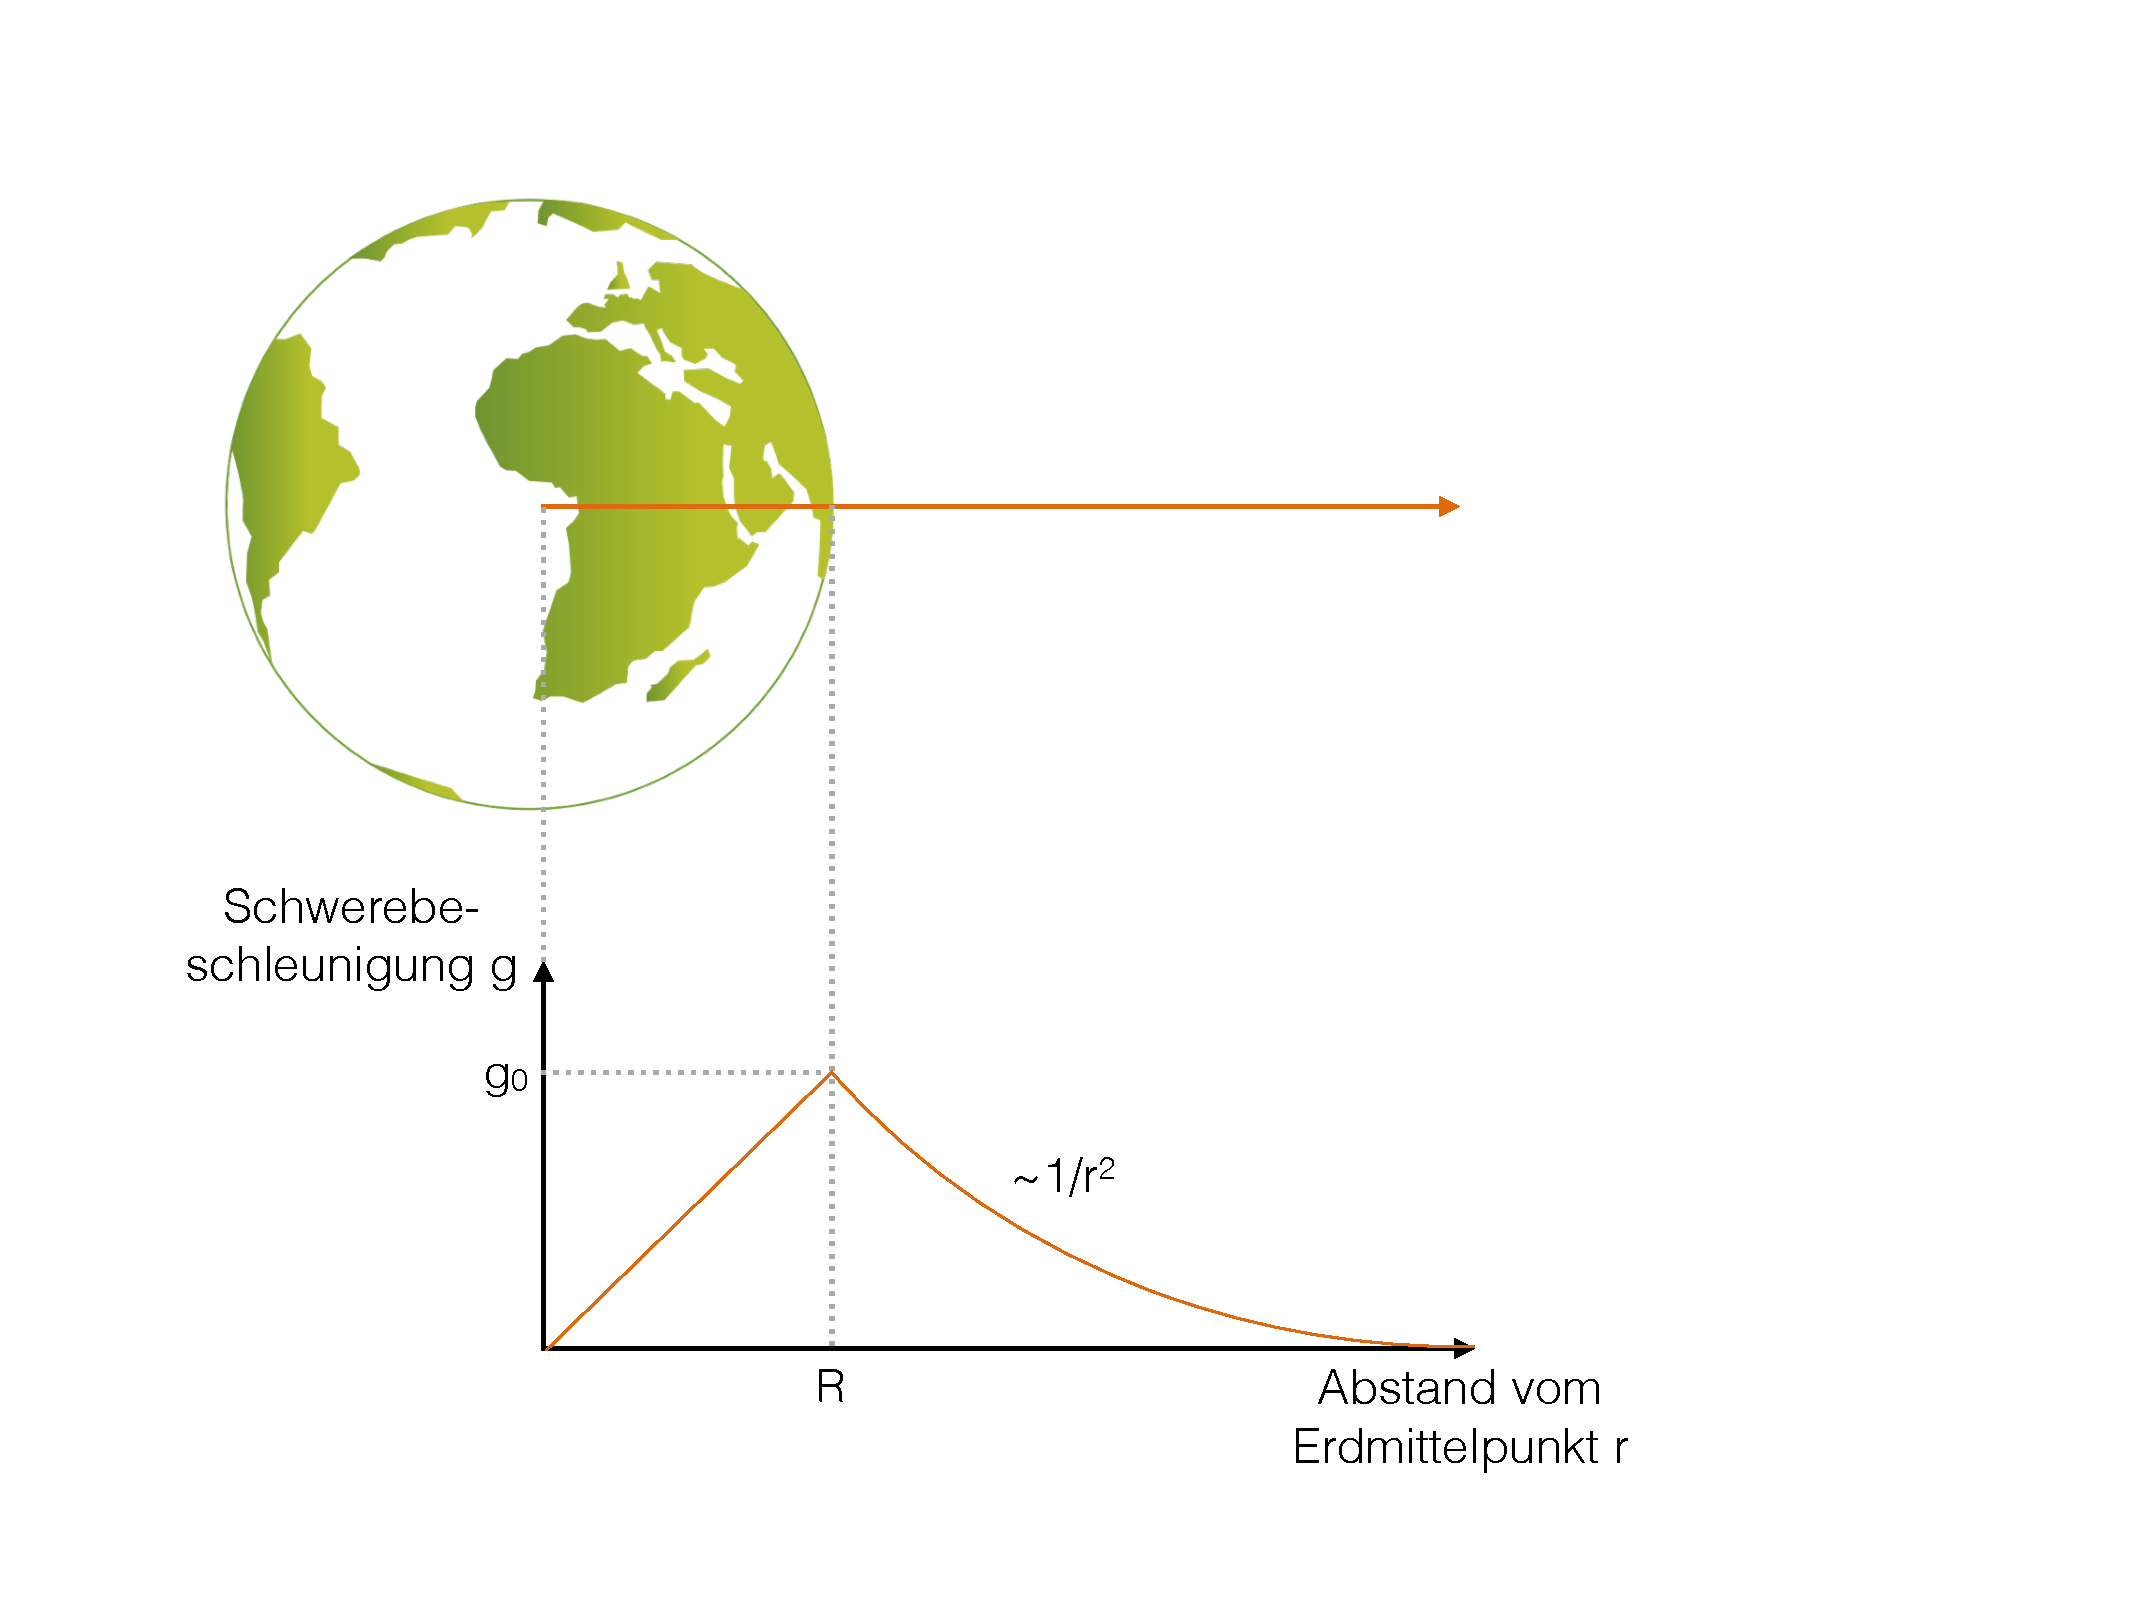
\includegraphics[width = \textwidth]{GravimetrieBilder/Abnahme_Grav}
\end{figure}


\subsection*{Die Erde als Kugel}

Wie bereits genannt, haben wir für diese Berechnungen angenommen, dass die Erde eine perfekte Kugel ist. Dies ist aber nicht der Fall. Eine bessere Näherung wäre ein Ellipsoid, wie wir später noch sehen werden. Die Abweichungen vom Kugelmodell entstehen durch verschiedene Faktoren: 
\begin{itemize}
	\item Inhomogenität der Erde
	\item gravitativer Einfluss durch Planeten, Gestirne (z.B. Sonne, Mond)
	\item gravitativer Einfluss durch Luftmassen in der Atmosphäre
	\item Fliehkraft durch Erdrotation
\end{itemize} 


Betrachten wir einmal den Einfluss dieser Faktoren auf eine gravimetrische Messung.  \begin{itemize}
	\item gravitativer Einfluss Mond: $\approx 82\,\si{\mu Gal}$
	\item gravitativer Einfluss Sonne: $\approx 38\,\si{\mu Gal}$
	\item Luftmassen: bis zu $900\,\si{\mu Gal}$
\end{itemize}
Vergleicht man diese Werte mit der Normalbeschleunigung ($981\,\si{Gal}$) und der Genauigkeit eines Messgerätes ($\approx 1\,\si{\mu Gal}$), ist offensichtlich, dass diese Variationen bei der Auswertung nicht vernachlässigt werden dürfen.

Dabei sei noch darauf hingewiesen, dass die Effekte von Sonne und Mond tagesabhängig sind, während sich der Einfluss durch Luftmassen ständig verändert. 


Mit dem formgebenden Faktor Fliehkraft beschäftigen wir uns nun noch genauer.
 
\subsubsection*{Fliehkraft durch Erdrotation}

Da sich durch die Fliehkraft die Form der Erde von der Kugel abhebt, ändert sich auch die Berechnung der lokalen Schwerebeschleunigung: \begin{equation*}
	g(\varphi) = \frac{G \cdot M}{R^2} - \omega^2 \cdot R \cdot cos^2(\varphi)
\end{equation*} 
Den ersten Teil der Formel vor dem Minus kennen wir bereits als Normalschwere, der hintere Teil ist neu. Dieser Teil ist die Zentrifugalbeschleunigung in tangetiale Richtung, in Abhängigkeit von der geozentrischen Breite. Die Erklärung was das bedeutet und wie dieser Teil sich herleiten lässt schauen wir uns nun an. Dazu betrachten wir diese Grafik:  

\begin{figure}[H]
\centering
  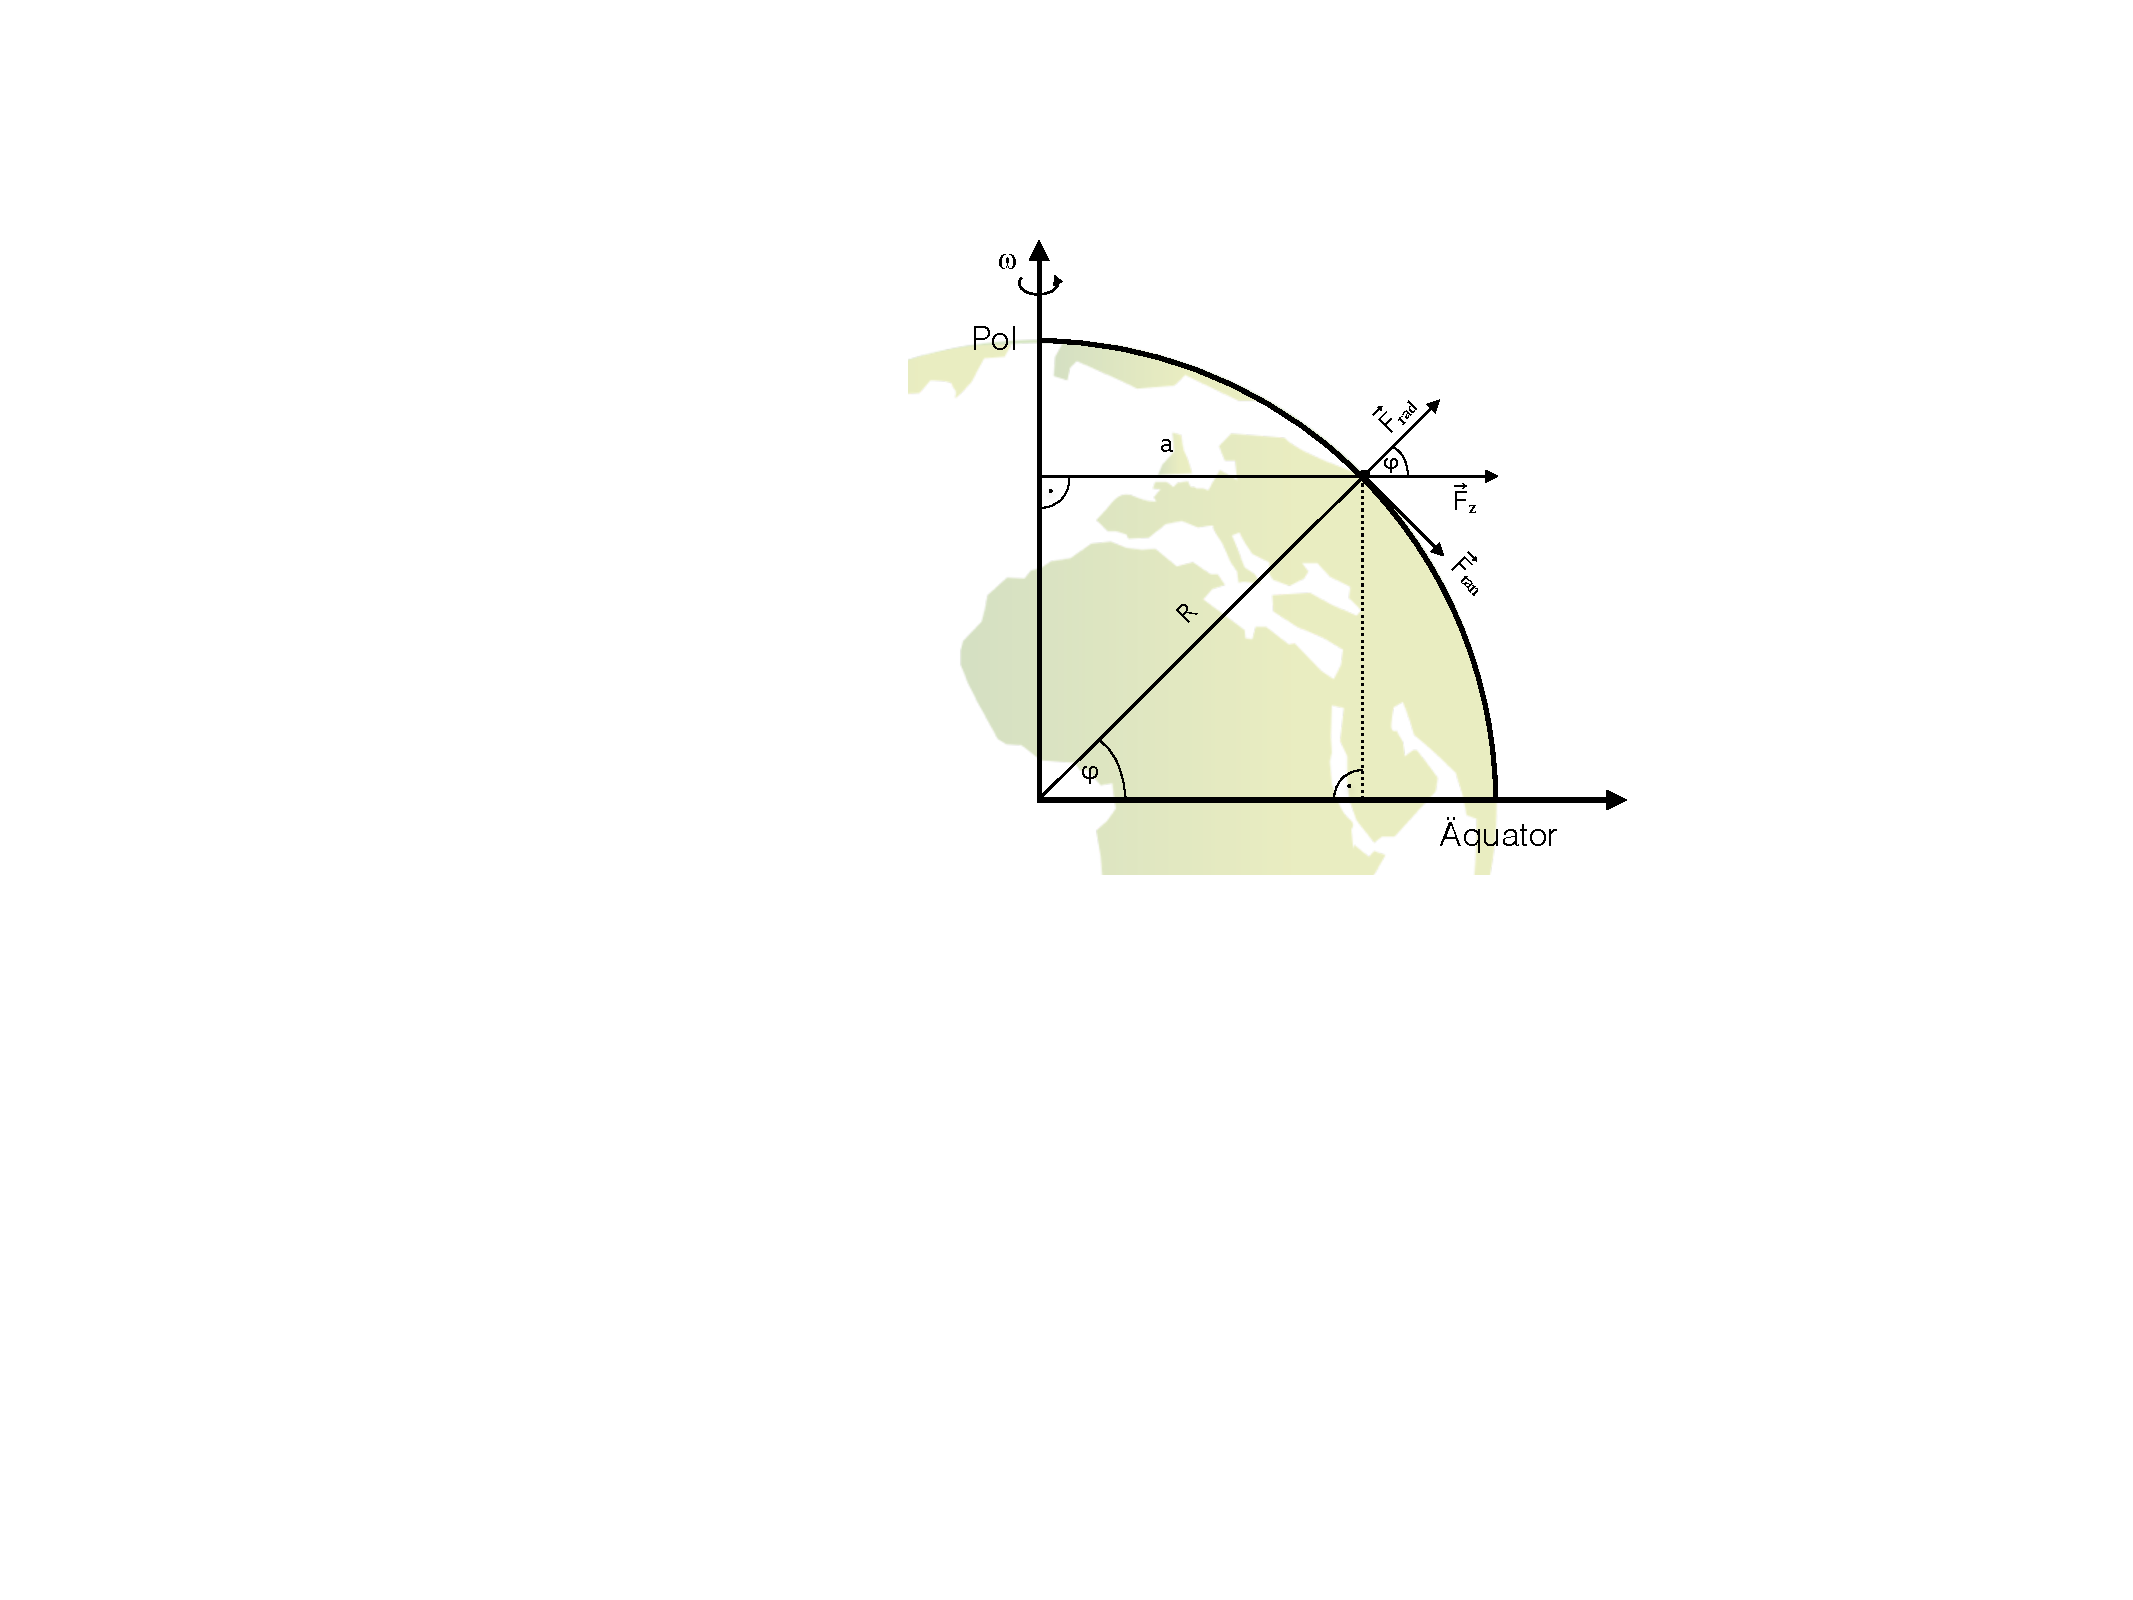
\includegraphics[width = \textwidth]{GravimetrieBilder/Fliehkraft}
\end{figure}

$\omega$ steht für die Drehgeschwindigkeit, also wie schnell sich die Erde um ihre eigene Achse dreht. Eine Umdrehung dauert, wie wir wissen, einen Tag. $\omega$ berechnet sich dann so: \begin{equation*}
	\omega = \frac{2 \pi}{1 \,\si{Tag}} = \frac{2 \pi}{24 \cdot 60 \cdot 60\,\si{s}} = \frac{2 \pi}{86400\,\si{s}} \approx 7,29 \cdot 10^{-5}\,\si{\frac{rad}{s}}
\end{equation*}

Den direkten Abstand einer Masse an der Erdoberfläche bezeichnen wir mit $a$ und den Erdradius mit $R$. 
$\varphi$ gibt die geozentrische Breite an, also auf welchem Breitengrad wir uns befinden. Am Äquator ist $\varphi$ = 0, am Nordpol gilt $\varphi$ = 90. Karlsruhe liegt ungefähr bei 49° nördliche Breite.

Übrig bleiben nun noch die drei Kräfte, die wir uns jetzt noch anschauen wollen. 
Die Zentrifugalkraft $|\vec{F}_z|$  wirkt senkrecht zur Rotationsachse und beschleunigt ein Objekt von ihr weg. Wir kennen das beispielsweise aus einem Karussell. Berechnen lässt sich die Zentrifugalkraft folgendermaßen: \begin{equation*}
	|\vec{F}_z| = m \cdot a \cdot \omega^2 = m \cdot b \quad \text{mit} \quad b = a \cdot \omega^2  
\end{equation*} $b$ ist hierbei die Zentrifugalbeschleunigung. 

Nehmen wir nun einmal an, dass wir den Abstand $a$  zur Rotationsachse nicht kennen. Um die Zentrifugalkraft berechnen zu können ist er aber essenziell. Betrachten wir noch einmal das Schaubild, besonders die gepunktete Linie von der x-Achse zu unserer Masse auf der Erdoberfläche: \begin{equation*}
	a = R \cdot cos(\varphi) 
	\end{equation*} 
Damit lässt sich die Zentrifugalkraft auch schreiben als \begin{equation*}
	|\vec{F}_z| = m \cdot a \cdot \omega^2 = m \cdot R \cdot cos(\varphi) \cdot \omega^2
\end{equation*}
Uns interessiert aber eigentlich nicht die totale Zentrifugalkraft, sondern nur der radiale Anteil $\vec{F}_{\text{rad}}$ , da dieser die Abweichung des Radius von der Kugel angibt. Um diesen Anteil berechnen zu können, teilen wir $\vec{F}_z$ auf in den gesuchten radialen, und einen tangentialen Anteil, die senkrecht zueinander sind. Um dies umzusetzen machen wir wieder einfache geometrische Überlegungen. \begin{equation*}
	|\vec{F}_{\text{rad}}| = |\vec{F}_z| \cdot cos(\varphi) = m \cdot b \cdot cos(\varphi) = m \cdot \omega^2 \cdot R \cdot cos^2(\varphi) 
\end{equation*} Dabei ist $\omega^2 \cdot R \cdot cos^2(\varphi)$ die Zentrifugalbeschleunigung in radialer Richtung. 
Zur Vollständigkeit sei auch noch der tangentiale Anteil genannt:  \begin{equation*}
	|\vec{F}_{\text{tan}}| = \frac{\omega^2 \cdot R}{2} sin(2\varphi) \cdot m 
\end{equation*}

Wir kennen nun die Beschleunigung der Erde durch Rotation in tangentiale Richtung und können damit die Schwerebeschleunigung auf einer rotierenden Kugel berechnen:  \begin{equation*}
	g(\varphi) = \frac{G \cdot M}{R^2} - \omega^2 \cdot R \cdot cos^2(\varphi) 
\end{equation*}

\subsection*{Näherungen an die Figur der Erde}
\subsubsection{(1) Kugel}
Die Näherung als Kugel haben wir bereits kennen gelernt. 

\subsubsection{(2) Referenzellipsoid}
Wählt man die Ellipse als Erdmodell, beachtet man die Verformung durch Fliehkräfte. Dadurch wird der Abstand von Pol zu Pol kleiner als die Hauptachse der Ellipse. Die jeweiligen Abweichungen von der Kugelerde sind jedoch relativ gering. 

\begin{figure}[H]
	\begin{subfigure}[m]{0.5\textwidth}
	\centering
		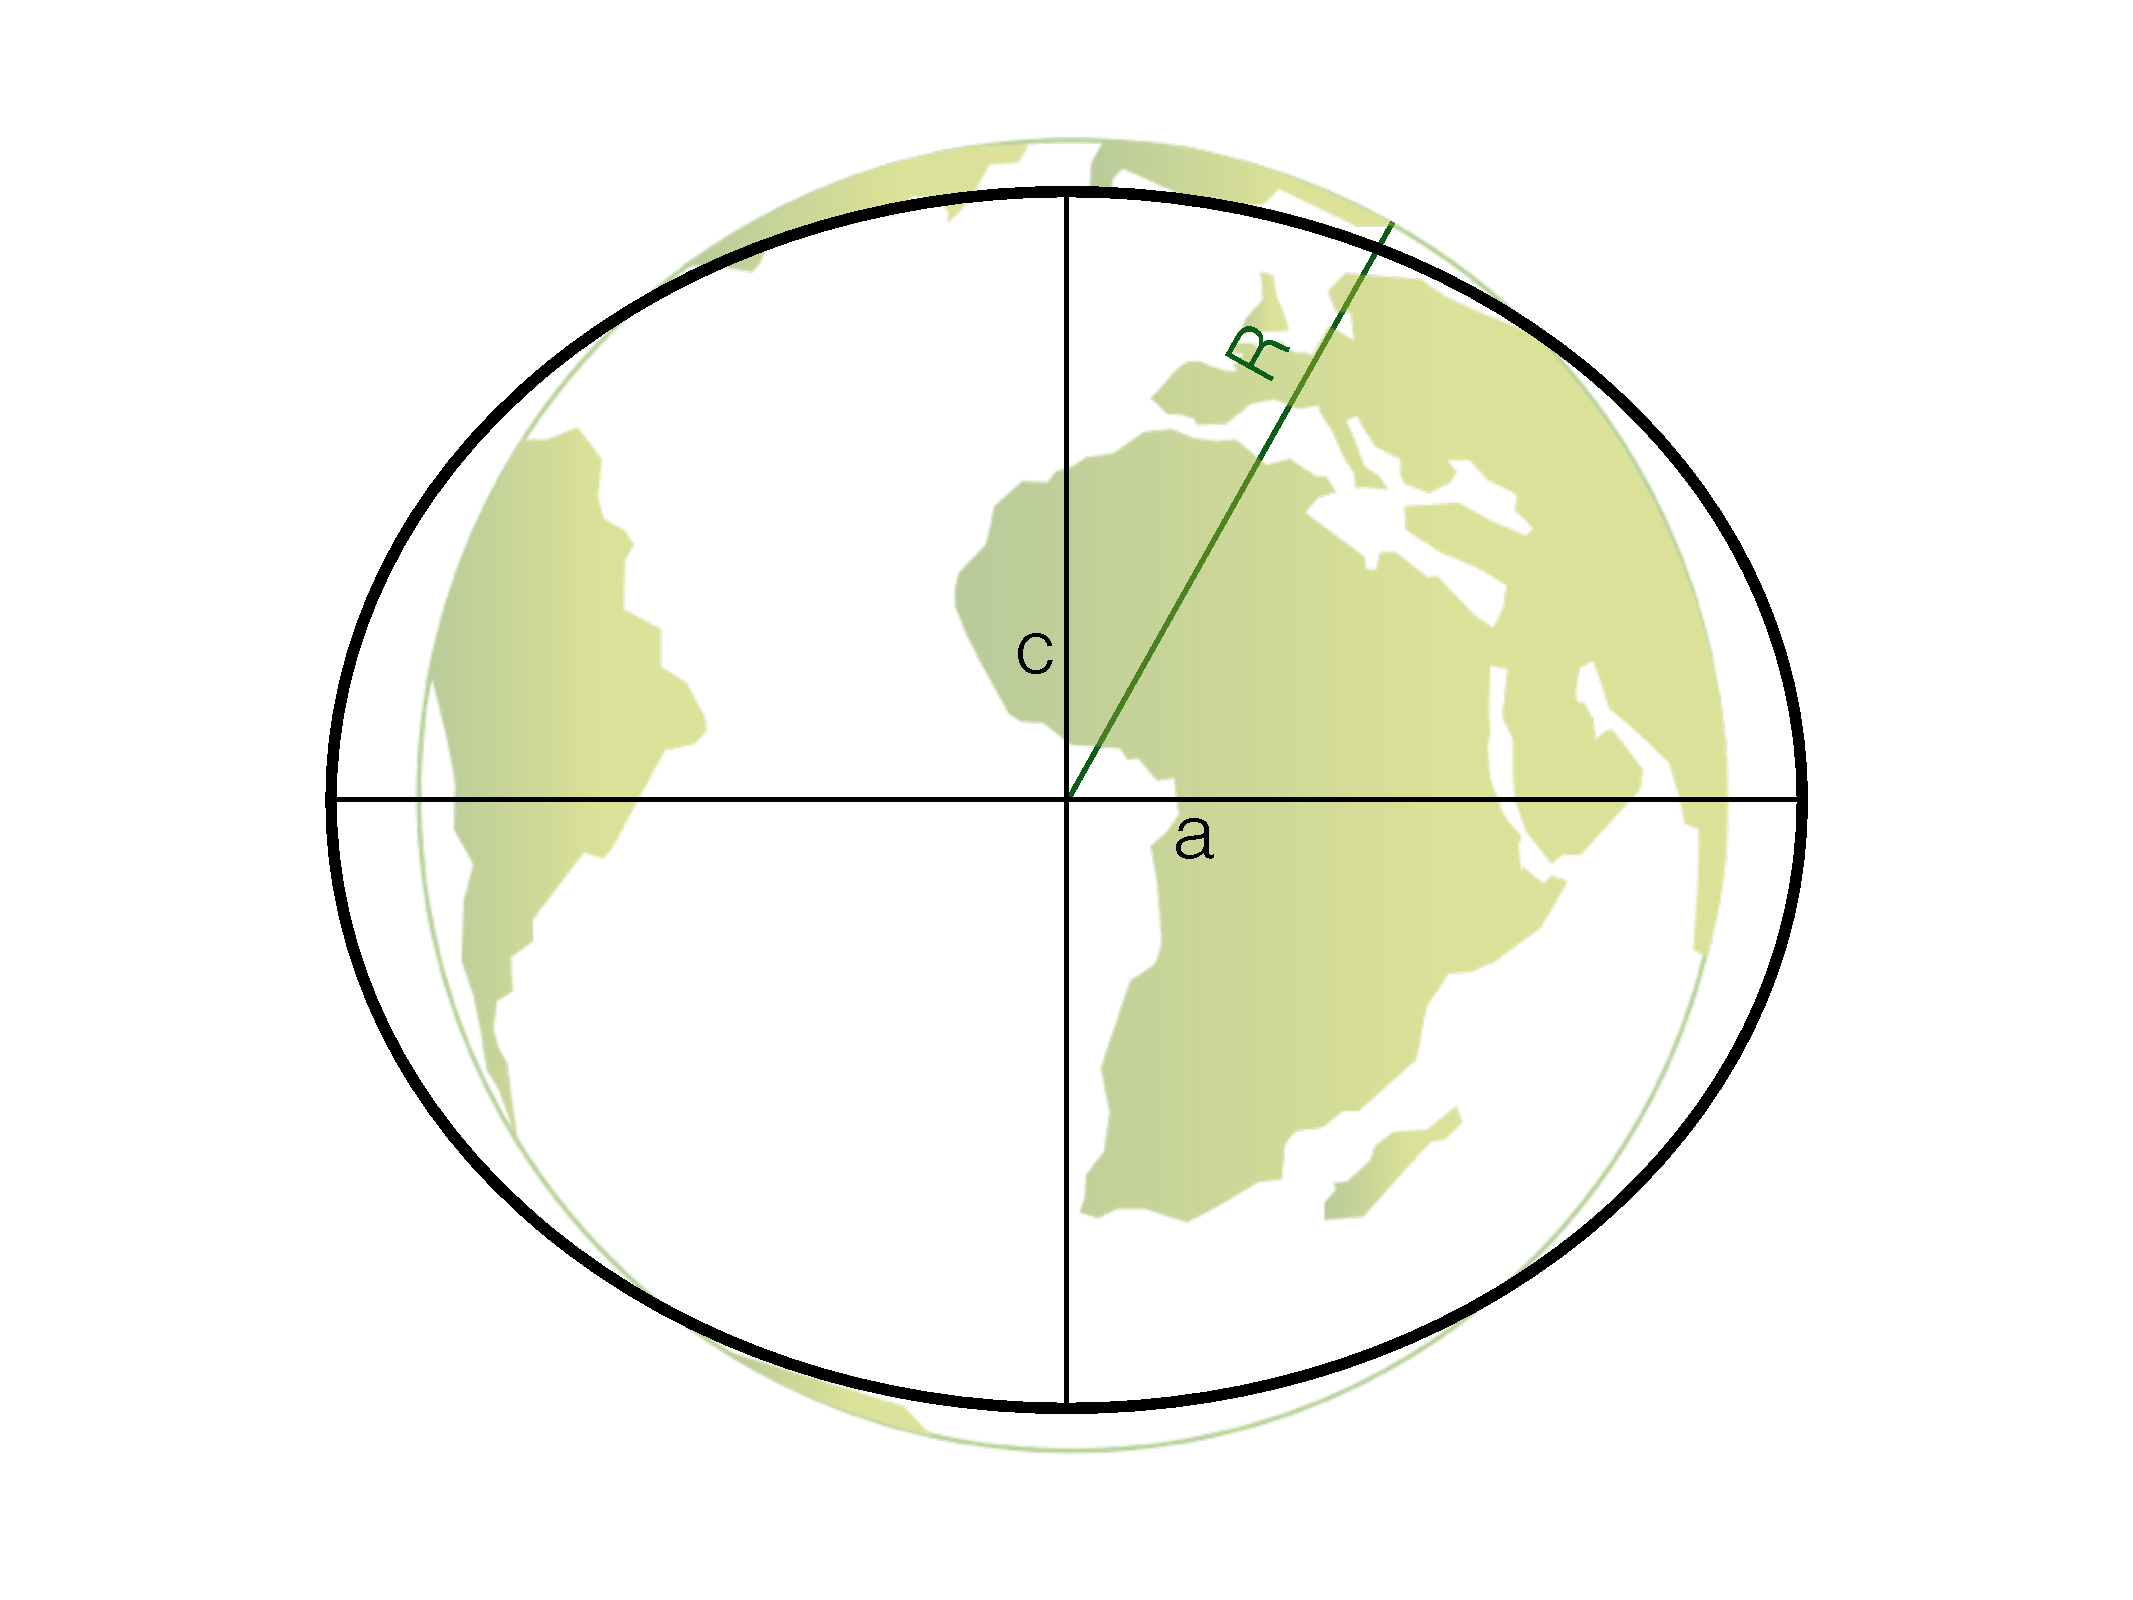
\includegraphics[scale=0.2]{GravimetrieBilder/Referenzellipsoid}
	\end{subfigure}
	\begin{subfigure}[m]{0.5\textwidth}
	\centering
		\[\begin{aligned}
			a &= 6378,136\,\si{km}\\
	c &= 6356, 751\,\si{km}\\
	R - a &\approx 7\,\si{km}\\
	R - c &\approx 15\,\si{km}
		\end{aligned}\]
	\end{subfigure}
\end{figure}

\subsubsection{(3) Geoid}
Die Gravitationskraft auf der Erde, also die Schwerkraft ist eine konservative Kraft. Das bedeutet zum einen, dass es ein Potential zur Kraft gibt. Dieses Schwerepotential $W$ wird über den Gradienten und das Vektorfeld der Schwerebeschleunigung definiert.
\begin{equation*}
	\vec{g} = - \text{grad}(W) = \left( \frac{\partial W}{\partial x}, \frac{\partial W}{\partial y}, \frac{\partial W}{\partial z} \right)^{\text{T}}	
\end{equation*} 
Weiterhin bedeutet es aber auch, dass es Äquipotentialflächen der Schwerebeschleunigung gibt. Anschaulich:

\begin{figure}[H]
	\centering
	\includegraphics[width = \textwidth]{GravimetrieBilder/Äquipotentialflächen}
\end{figure}
Entlang solcher Flächen erfordert das Bewegen einer Masse keine Arbeit. 

Die Oberflächen ruhender Ozeane oder Seen sind solche Äqupotentialflächen. Als Geoid bezeichnet man nun die Äquipotentialfläche, die dem mittleren Niveau aller Ozeane entspricht. Es gilt also \begin{equation*}
	W = W_{\text{Geoid}} = \text{konst.}
\end{equation*}

\begin{figure}[H]
	\centering
	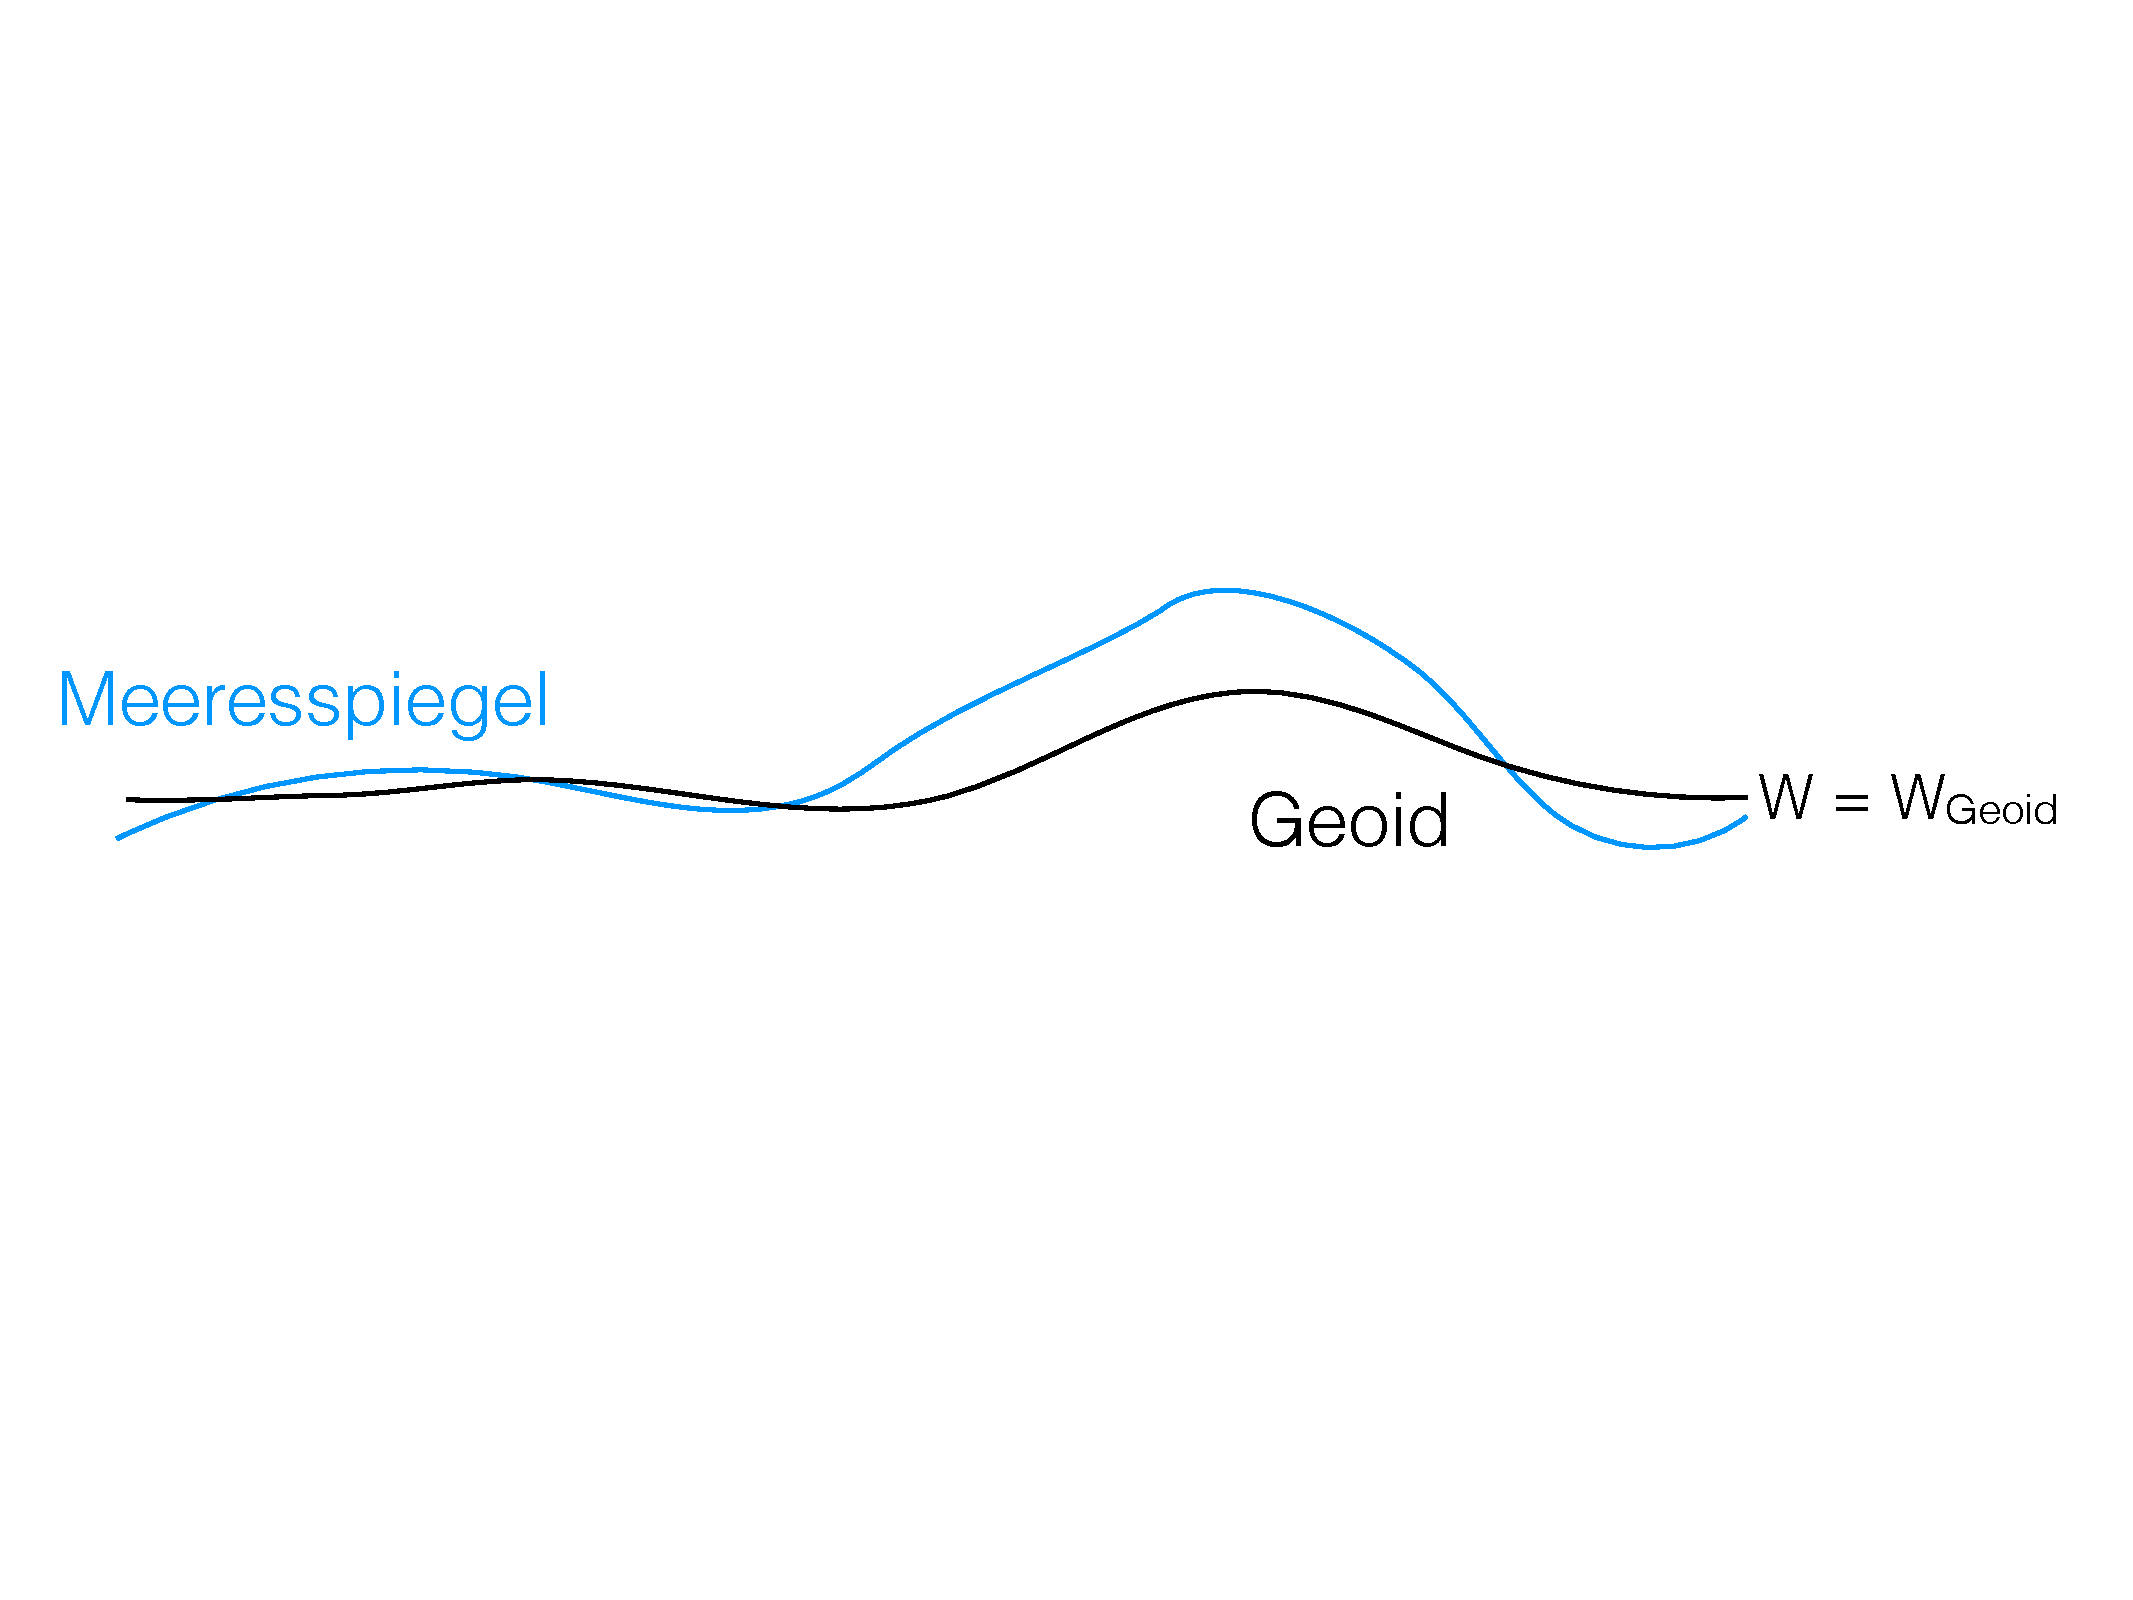
\includegraphics[width = \textwidth]{GravimetrieBilder/Geoid}
\end{figure}

Abweichungen des Geoid vom Referenzellipsoiden werden als Geoidundulationen bezeichnet. Diese Abweichungen bewegen sich zwischen etwa -105\,m im nördlichen indischen Ozean und ungefähr +70\,m nördlich von Papua-Neuguinea. 

\begin{figure}[H]
  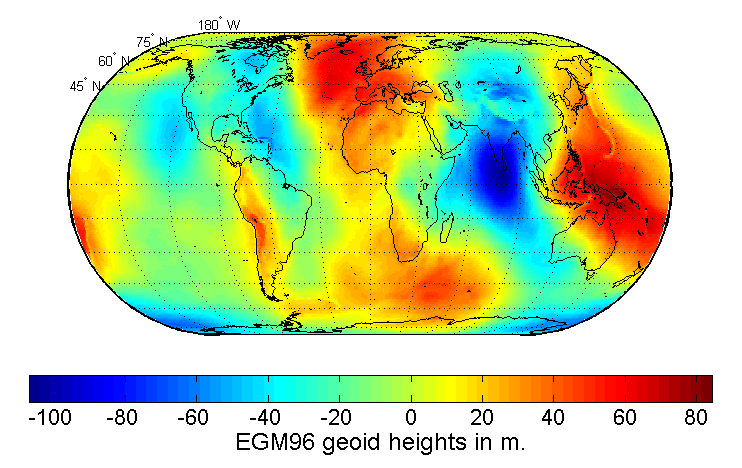
\includegraphics[width = \textwidth]{GravimetrieBilder/Geoidundulation}
  \caption*{Globale Geoidundulation. \textit{Quelle: Wikipedia}}
\end{figure}

Es sei noch darauf hingewiesen, dass für gravimetrische Messungen die Erde als Kugel bzw. als Ellipsoid angenähert wird. Zwar wäre ein Geoid die richtige Näherung, aber sie lässt sich nur schwer mathematisch beschreiben und eignet sich für das Berechnen der Schwerekorrekturen daher nicht. 


\section{Schwerereduktionen}

\begin{figure}[H]
	\centering
	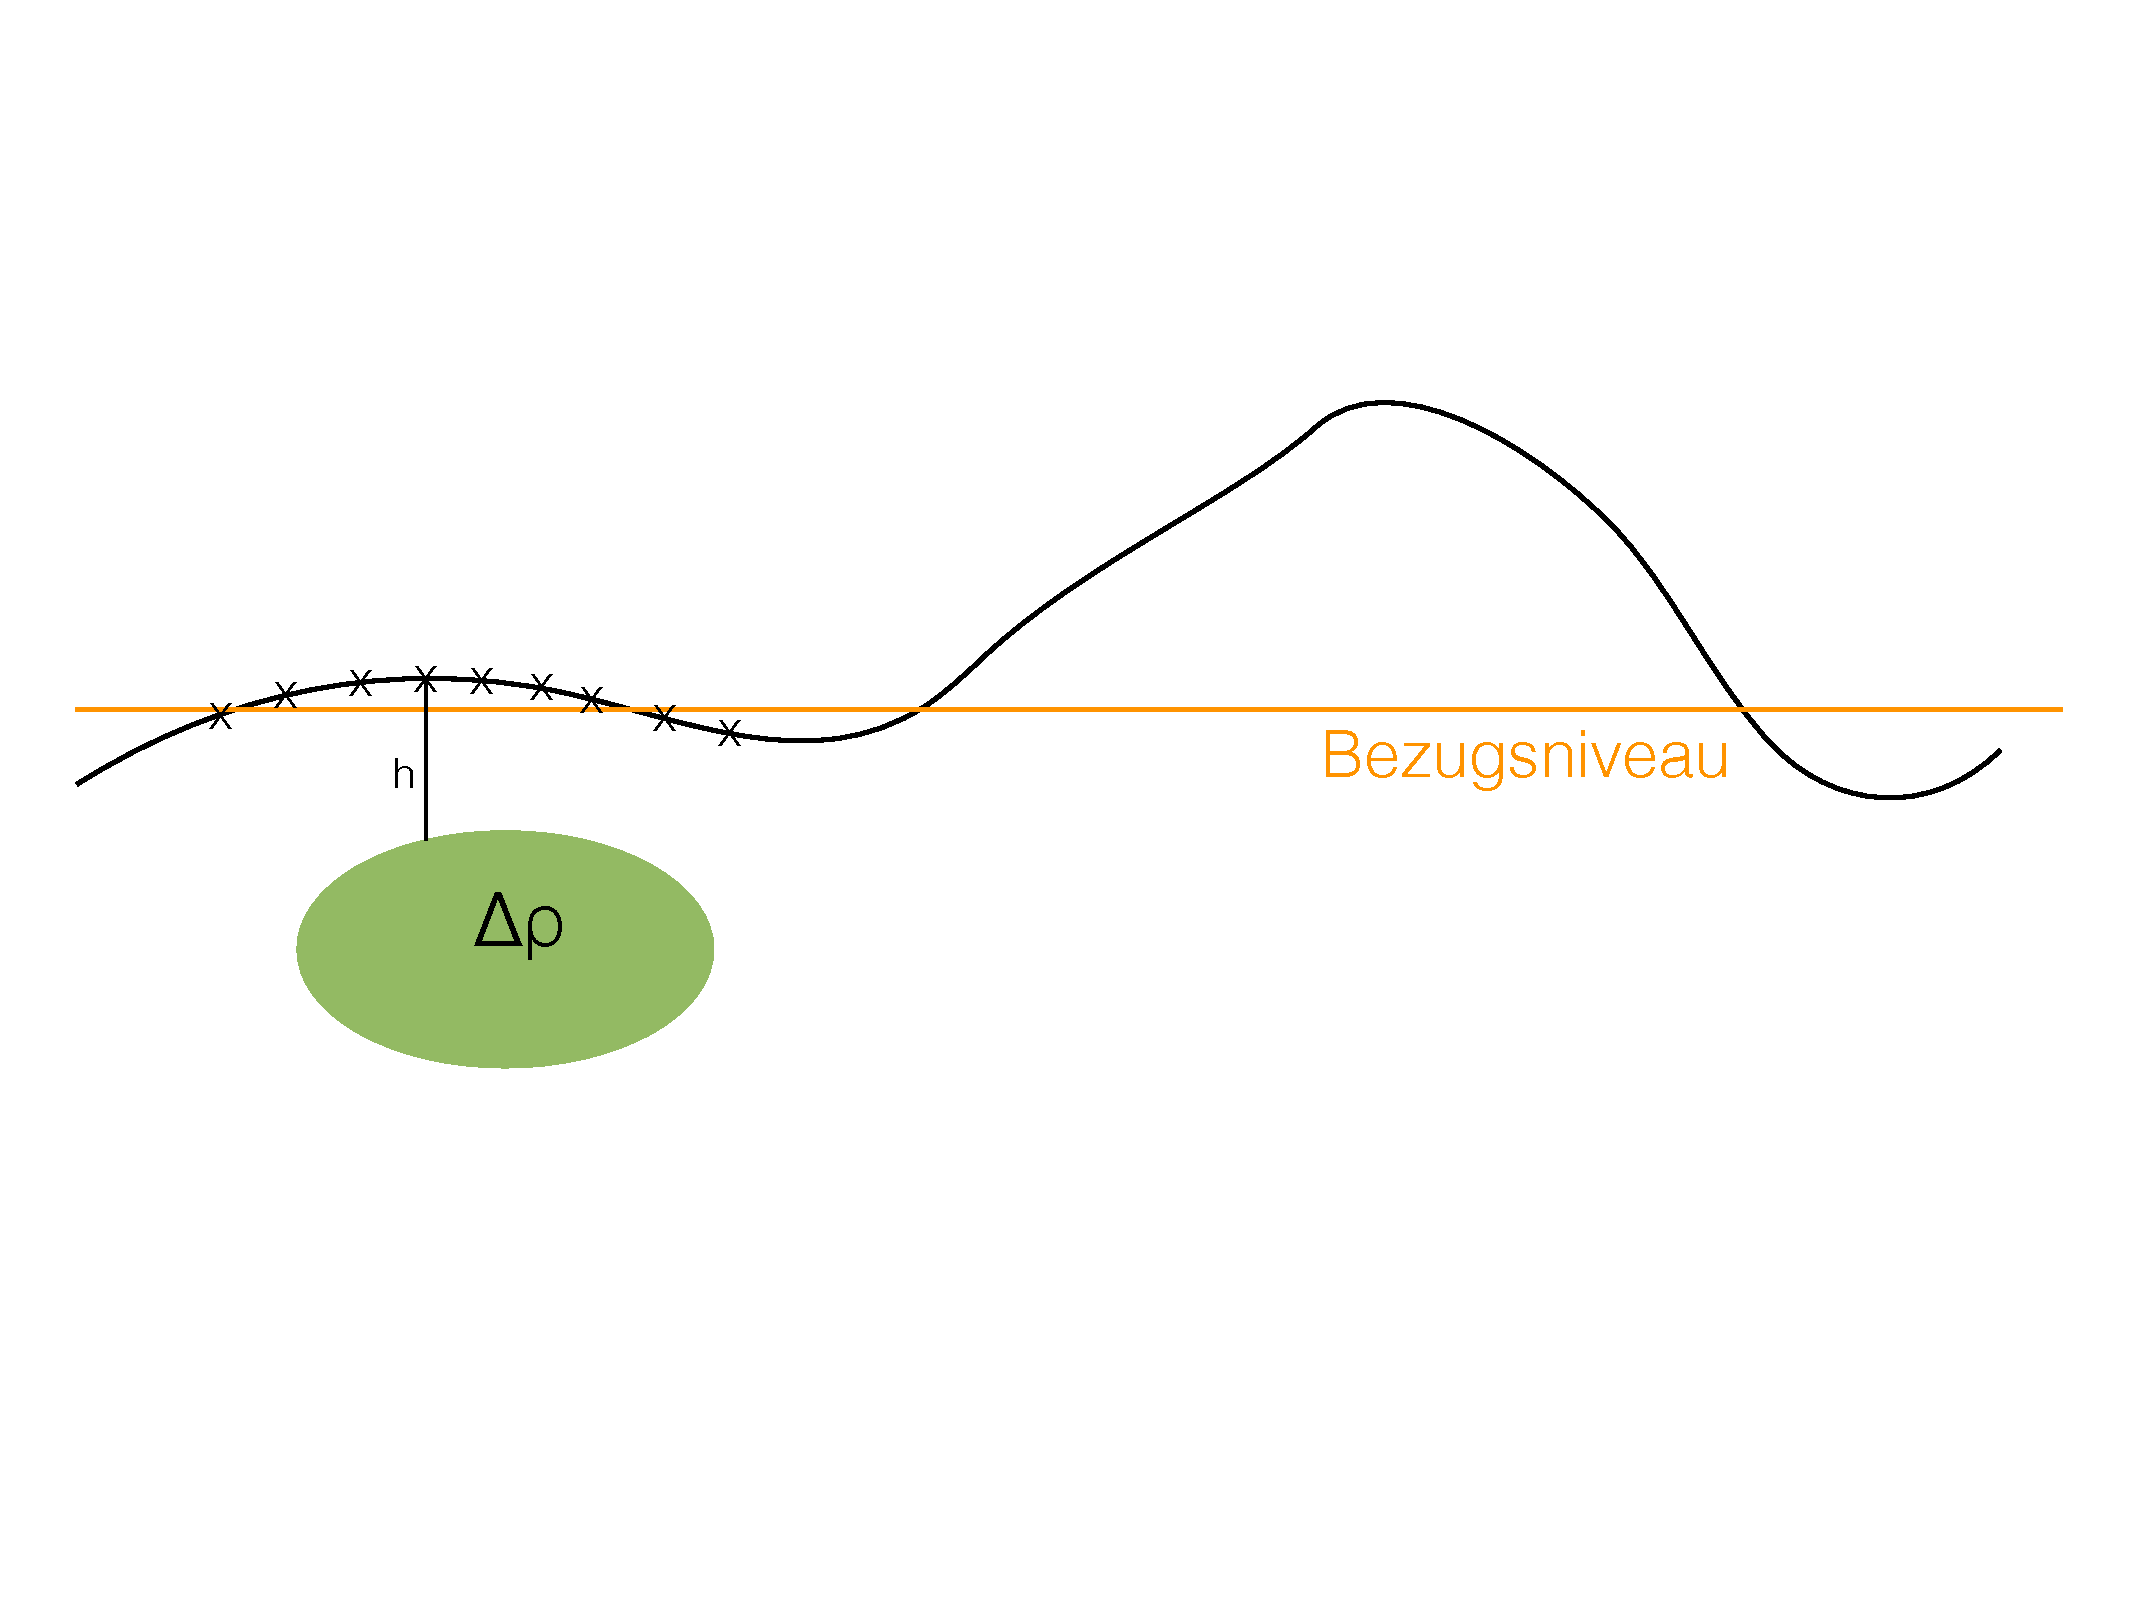
\includegraphics[width = \textwidth]{GravimetrieBilder/Schwerereduktionen}
\end{figure}

Das Ziel einer gravimetrischen Messung ist die Darstellung einer lokalen Schwereanomalie im Untergrund, die durch Dichteanomalien (Grafik: $\Delta \rho$) hervorgerufen wird. Da die Messgeräte hoch empfindlich sind müssen diverse Störfaktoren der Umwelt und Umgebung korrigiert werden. Diese Korrekturen werden unabhängig voneinander berechnet.  
\begin{enumerate}
	\item Wirkung der gesamten Erde \begin{itemize}
		\item Normalschwerereduktion $\gamma_0$
		\item Wirkung der Zentrifugalbeschleunigung (abhängig von geographischer Breite): Breitenreduktion $\delta_{\gamma_0}$
		\end{itemize}
	\item Höhenunterschiede: Freiluftreduktion $\delta_{g_{FL}}$
	\item Wirkung der Gesteinsmasse: Bouger-Reduktion $\delta_{g_B}$
	\item Topographie der Umgebung: Topographische Reduktion $\delta_{g_{\text{Top}}}$
	\item Zeitabhängige Faktoren: Gerätegang, Gezeiten,\dots \space$g(t)$
\end{enumerate} 
Die Schwereanomalie errechnet sich dann mit folgender Formel: 
\begin{equation*}
	\Delta g = g(x,y,z,t) - g(t) - \delta_g (x,y,z)
\end{equation*}
Dabei ist $g(x,y,z,t)$ die gemessene Schwerebeschleunigung, $g(t)$ sind die zeitabhängigen Faktoren und $\delta_g (x,y,z)$ die ortsabhängigen Faktoren. 
Im Folgenden werden wir die ortsabhängigen Faktoren und ihre Berechnung genauer betrachten. 

\subsection{Wirkung der gesamten Erde}
\subsubsection{Normalschwerereduktion}

\begin{description} 
	\item rotierende Kugel: Diese Formel kenn wir bereits aus Kapitel 7.2. Auch ihre Herleitung haben wir dort bereits betrachtet. \begin{equation*}
		\gamma_0 = g(\varphi) = \ub{\frac{G \cdot M}{R^2}}{\gamma_0} - \ub{\omega^2 \cdot R \cdot cos^2(\varphi_B)}{\substack{\text{Zentrifugal-} \\ \text{beschleunigung}}}
	\end{equation*}
	
	\item rotierendes Ellipsoid: \begin{equation*}
		\gamma_0 = g_{\text{Ellips.}} = 9,7803 \cdot (1 + 0,0053 \cdot sin^2(\varphi_B) - 5,8 \cdot 10^{-6} sin^2(\varphi_B))
	\end{equation*} Wir wollen nicht näher darauf eingehen wie diese Formel zustande kommt.
\end{description}

\subsubsection{Breitenreduktion} 
Aus der obigen Gleichung der Normalschwere für den Rotationsellipsoiden lässt sich die Breitenkorrektur berechnen. Diese ist abhängig von der geographischen Breite $\varphi_B$ des Referenzpunktes $R$, da die Schwerebeschleunigung auf dem Referenzellipsoiden in Richtung der Pole zunimmt. \begin{equation*}
	\delta_{\gamma_0} = 0,00081 \cdot sin^2(2 \cdot \varphi_B) \cdot \Delta y
\end{equation*}
$\Delta y$ bezeichnet hierbei die Abweichung des Messpunktes vom Referenzpunkt in Nord-Süd-Richtung in\,km. 

\begin{figure}[H]
	\centering
	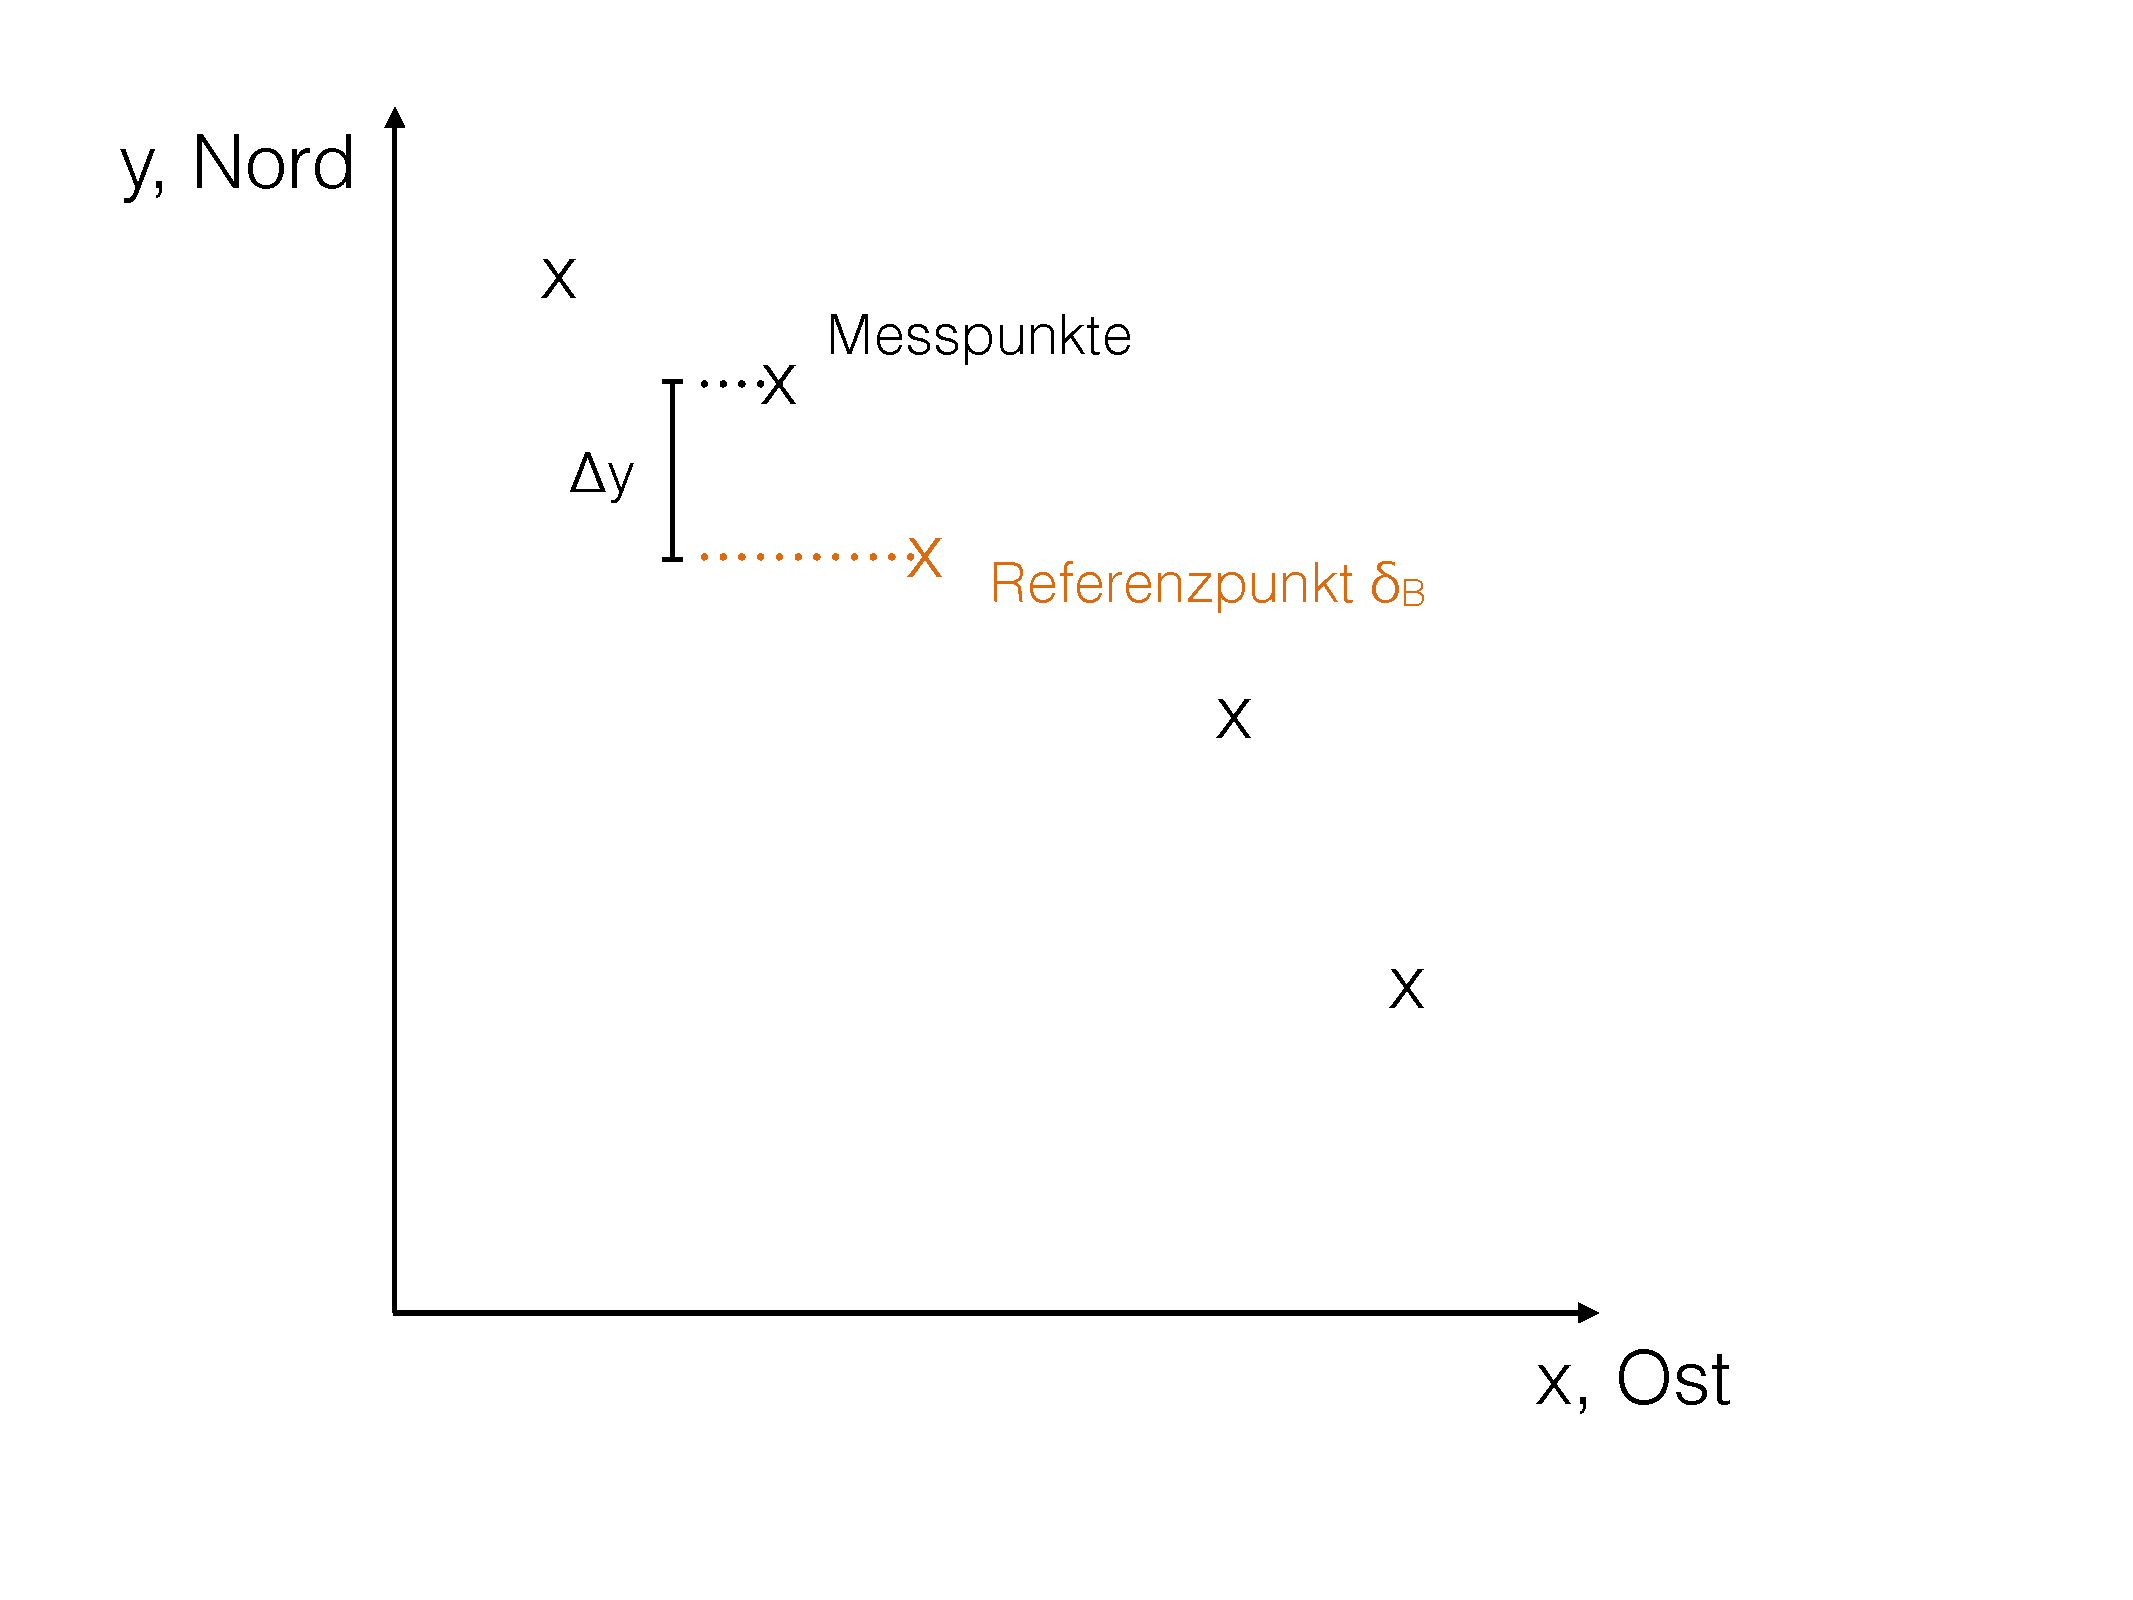
\includegraphics[scale = 0.3]{GravimetrieBilder/Breitenreduktion}
\end{figure}

\subsection{Freiluftreduktion}

\begin{figure}[H]
	\centering
	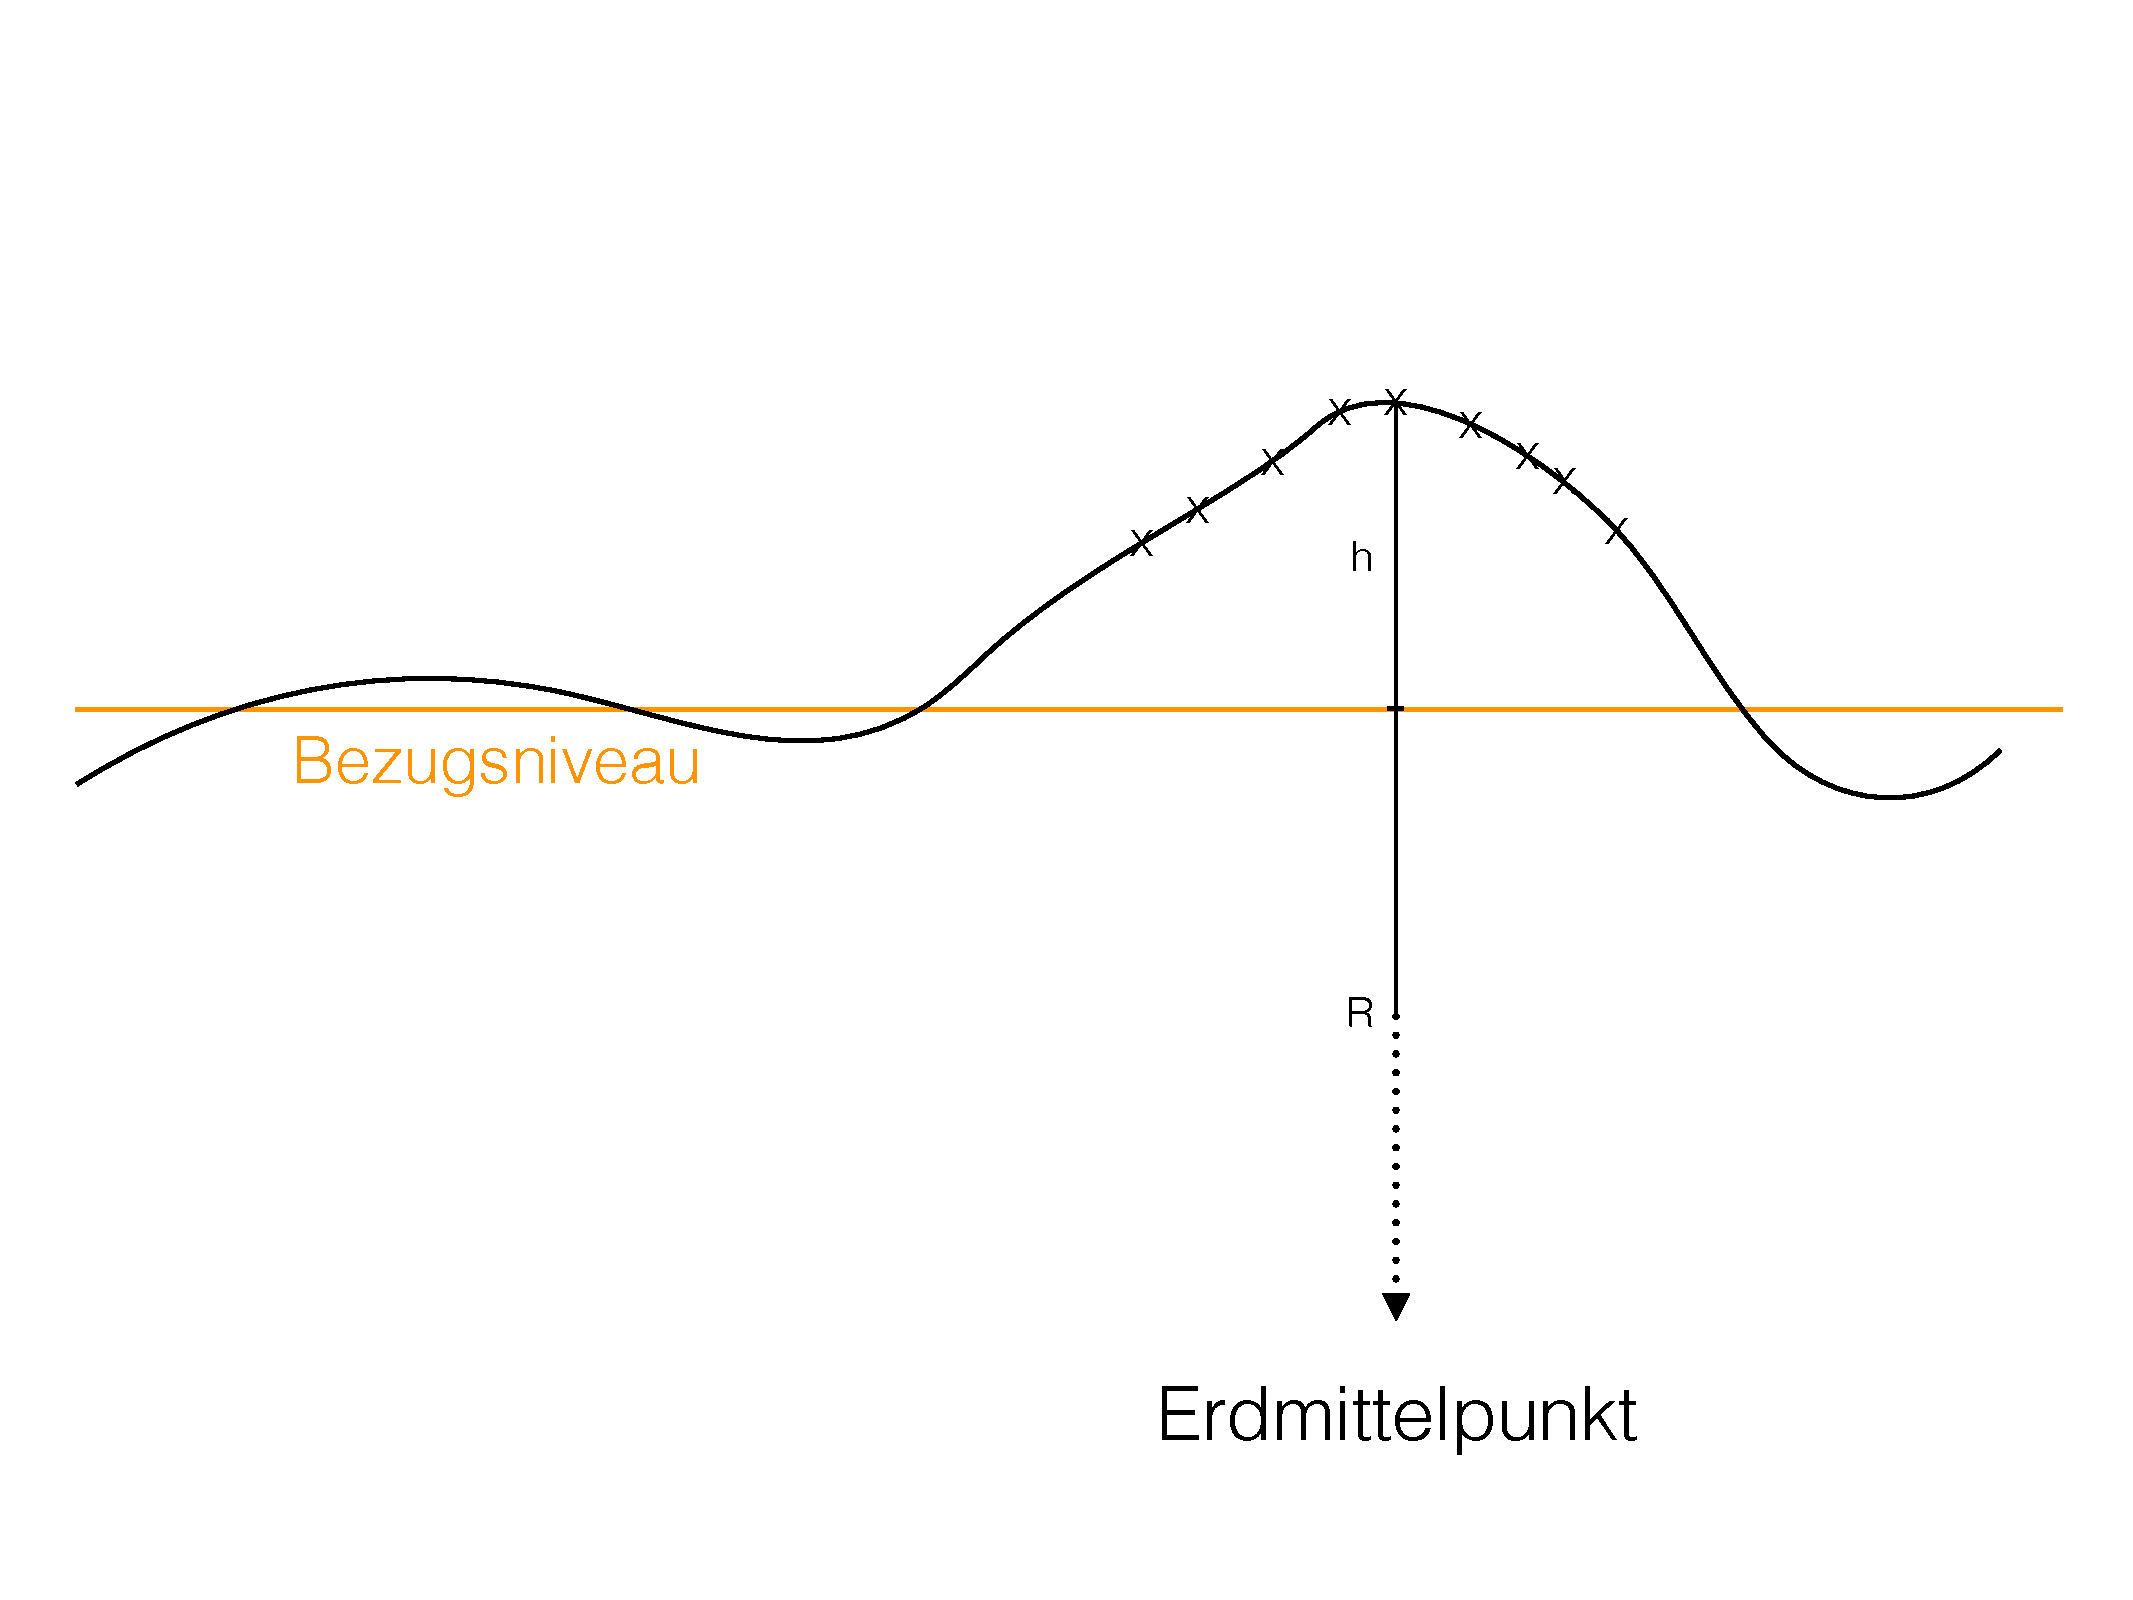
\includegraphics[width = \textwidth]{GravimetrieBilder/Freiluftreduktion}
\end{figure}

Bei einer gravimetrischen Messung wird ein Bezugsniveau festgelegt, auf das alle Messpunkte normiert werden. Dieses Bezugsniveau kann beispielsweise das Normalnull sein. Grund für eine Normierung ist der Abstand der Messpunkte vom Erdmittelpunkt, also unterschiedliche Radien. Die Schwerebeschleunigung nimmt aber mit höherem Radius ab. Diesen Unterschied gleicht man mit der Freiluftkorrektur aus. \begin{align*}
	\delta_{g_{FL}} &= G \cdot \left( \frac{M}{(R + h)^2} - \frac{M}{R^2} \right) \\
	&\approx -2 \cdot \frac{G \cdot M}{R^2} \cdot \frac{h}{R} = -2 \cdot \gamma_0 \frac{h}{R} \approx -0,3086 \cdot h\,\si{m Gal}
\end{align*}
Die Höhenmessung wird mit DGPS durchgeführt und hat eine Genauigkeit von ungefähr 3\,cm: \begin{equation*}
	\Delta (\delta_{g_{FL}}) \leq 0,01\,\si{m Gal} \quad \Rightarrow \quad \Delta h = \frac{1}{0,3086} \cdot \Delta (\delta_{g_{FL}}) \approx 0,03\,\si{m}
\end{equation*}
\subsubsection{Freiluftanomalie} 
Die Freiluftanomalie ist eine erste Berechnung der Dichteanomalie im Untergrund. Bei dieser Anomalie sind zusätzlich zu den zeitabhängigen Faktoren nur Normalschwerereduktion und Höhenkorrektur mit eingerechnet. \begin{equation*}
	\Delta g_{FL} = g(x, y, z, t) - g(t) - \gamma_0 - \delta_{\gamma_0} - \delta_{g_{FL}}
\end{equation*}

\subsection{Bouguer-Reduktion}
Bringt man die Messpunkte auf ein Bezugsniveau, muss nicht nur die Schwereveränderung durch die Höhe, sondern auch die Schwerewirkung der zwischenliegenden Gesteinsmasse eingerechnet werden. 

\begin{figure}[H]
	\centering
	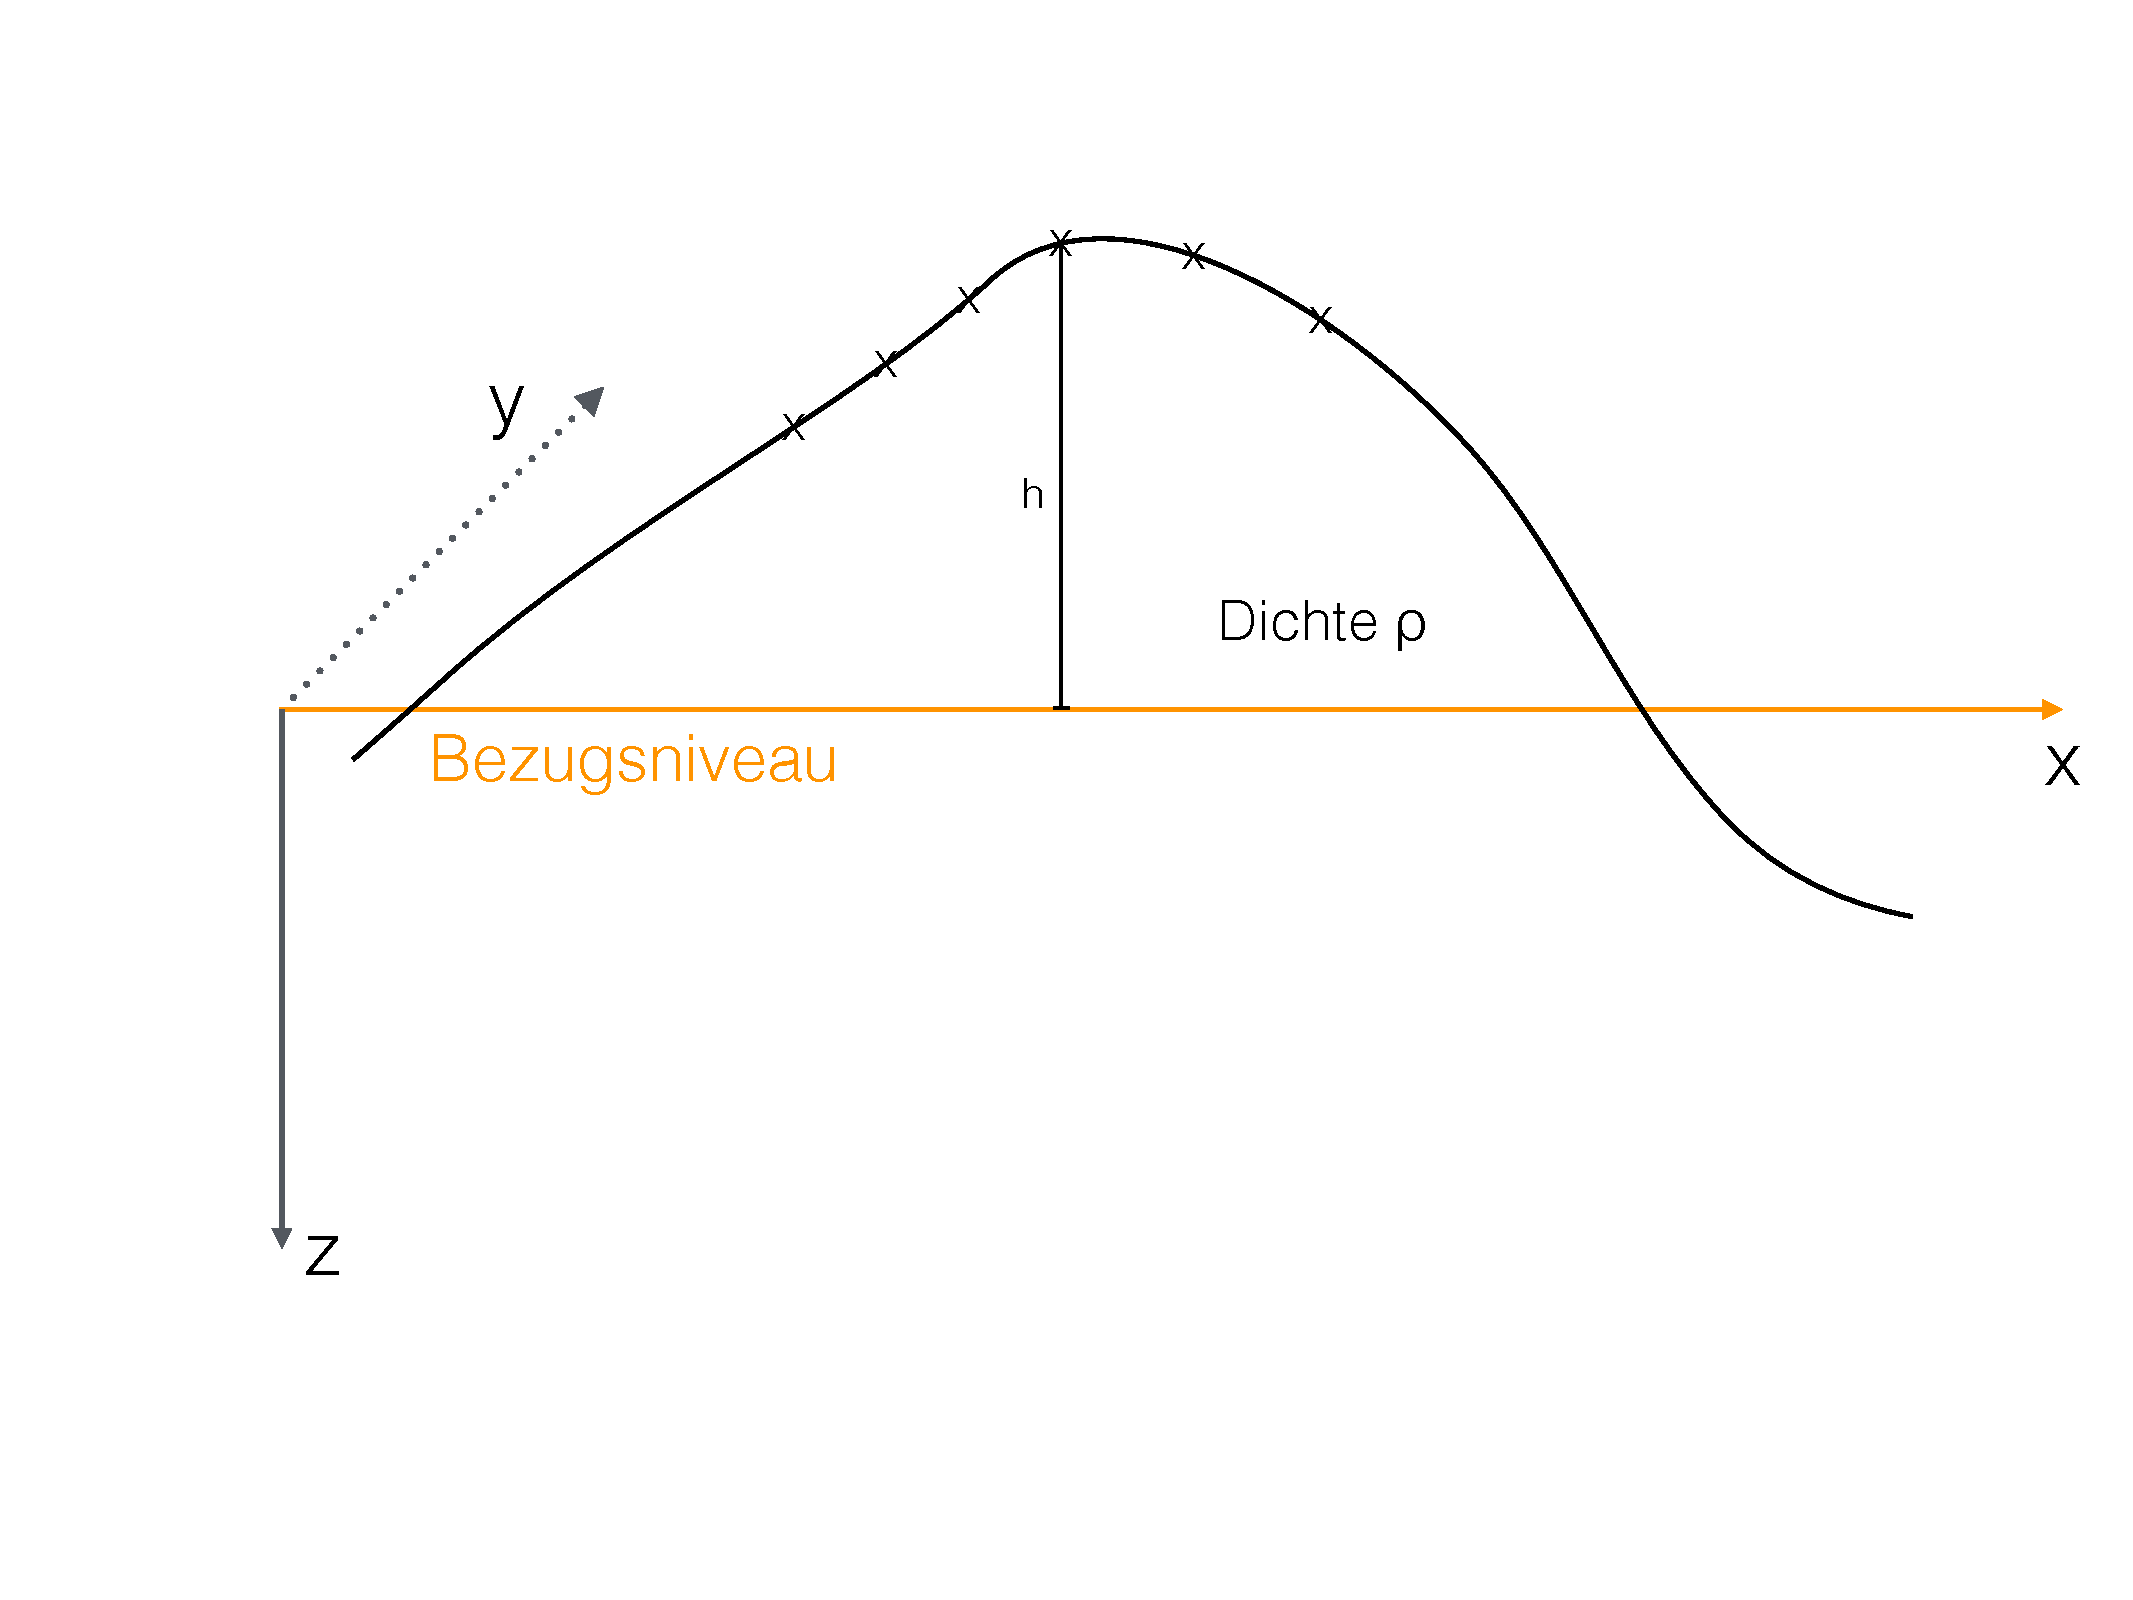
\includegraphics[width = \textwidth]{GravimetrieBilder/Bouguer-Reduktion1}
\end{figure}

Diese Gesteinsmasse wird als Platte angenähert, die in alle Seiten ins unendliche ausgedehnt ist und Mächtigkeit (Reduktionshöhe) $h$ und homogene Massendichte $\rho$ hat. 

\begin{figure}[H]
	\centering
	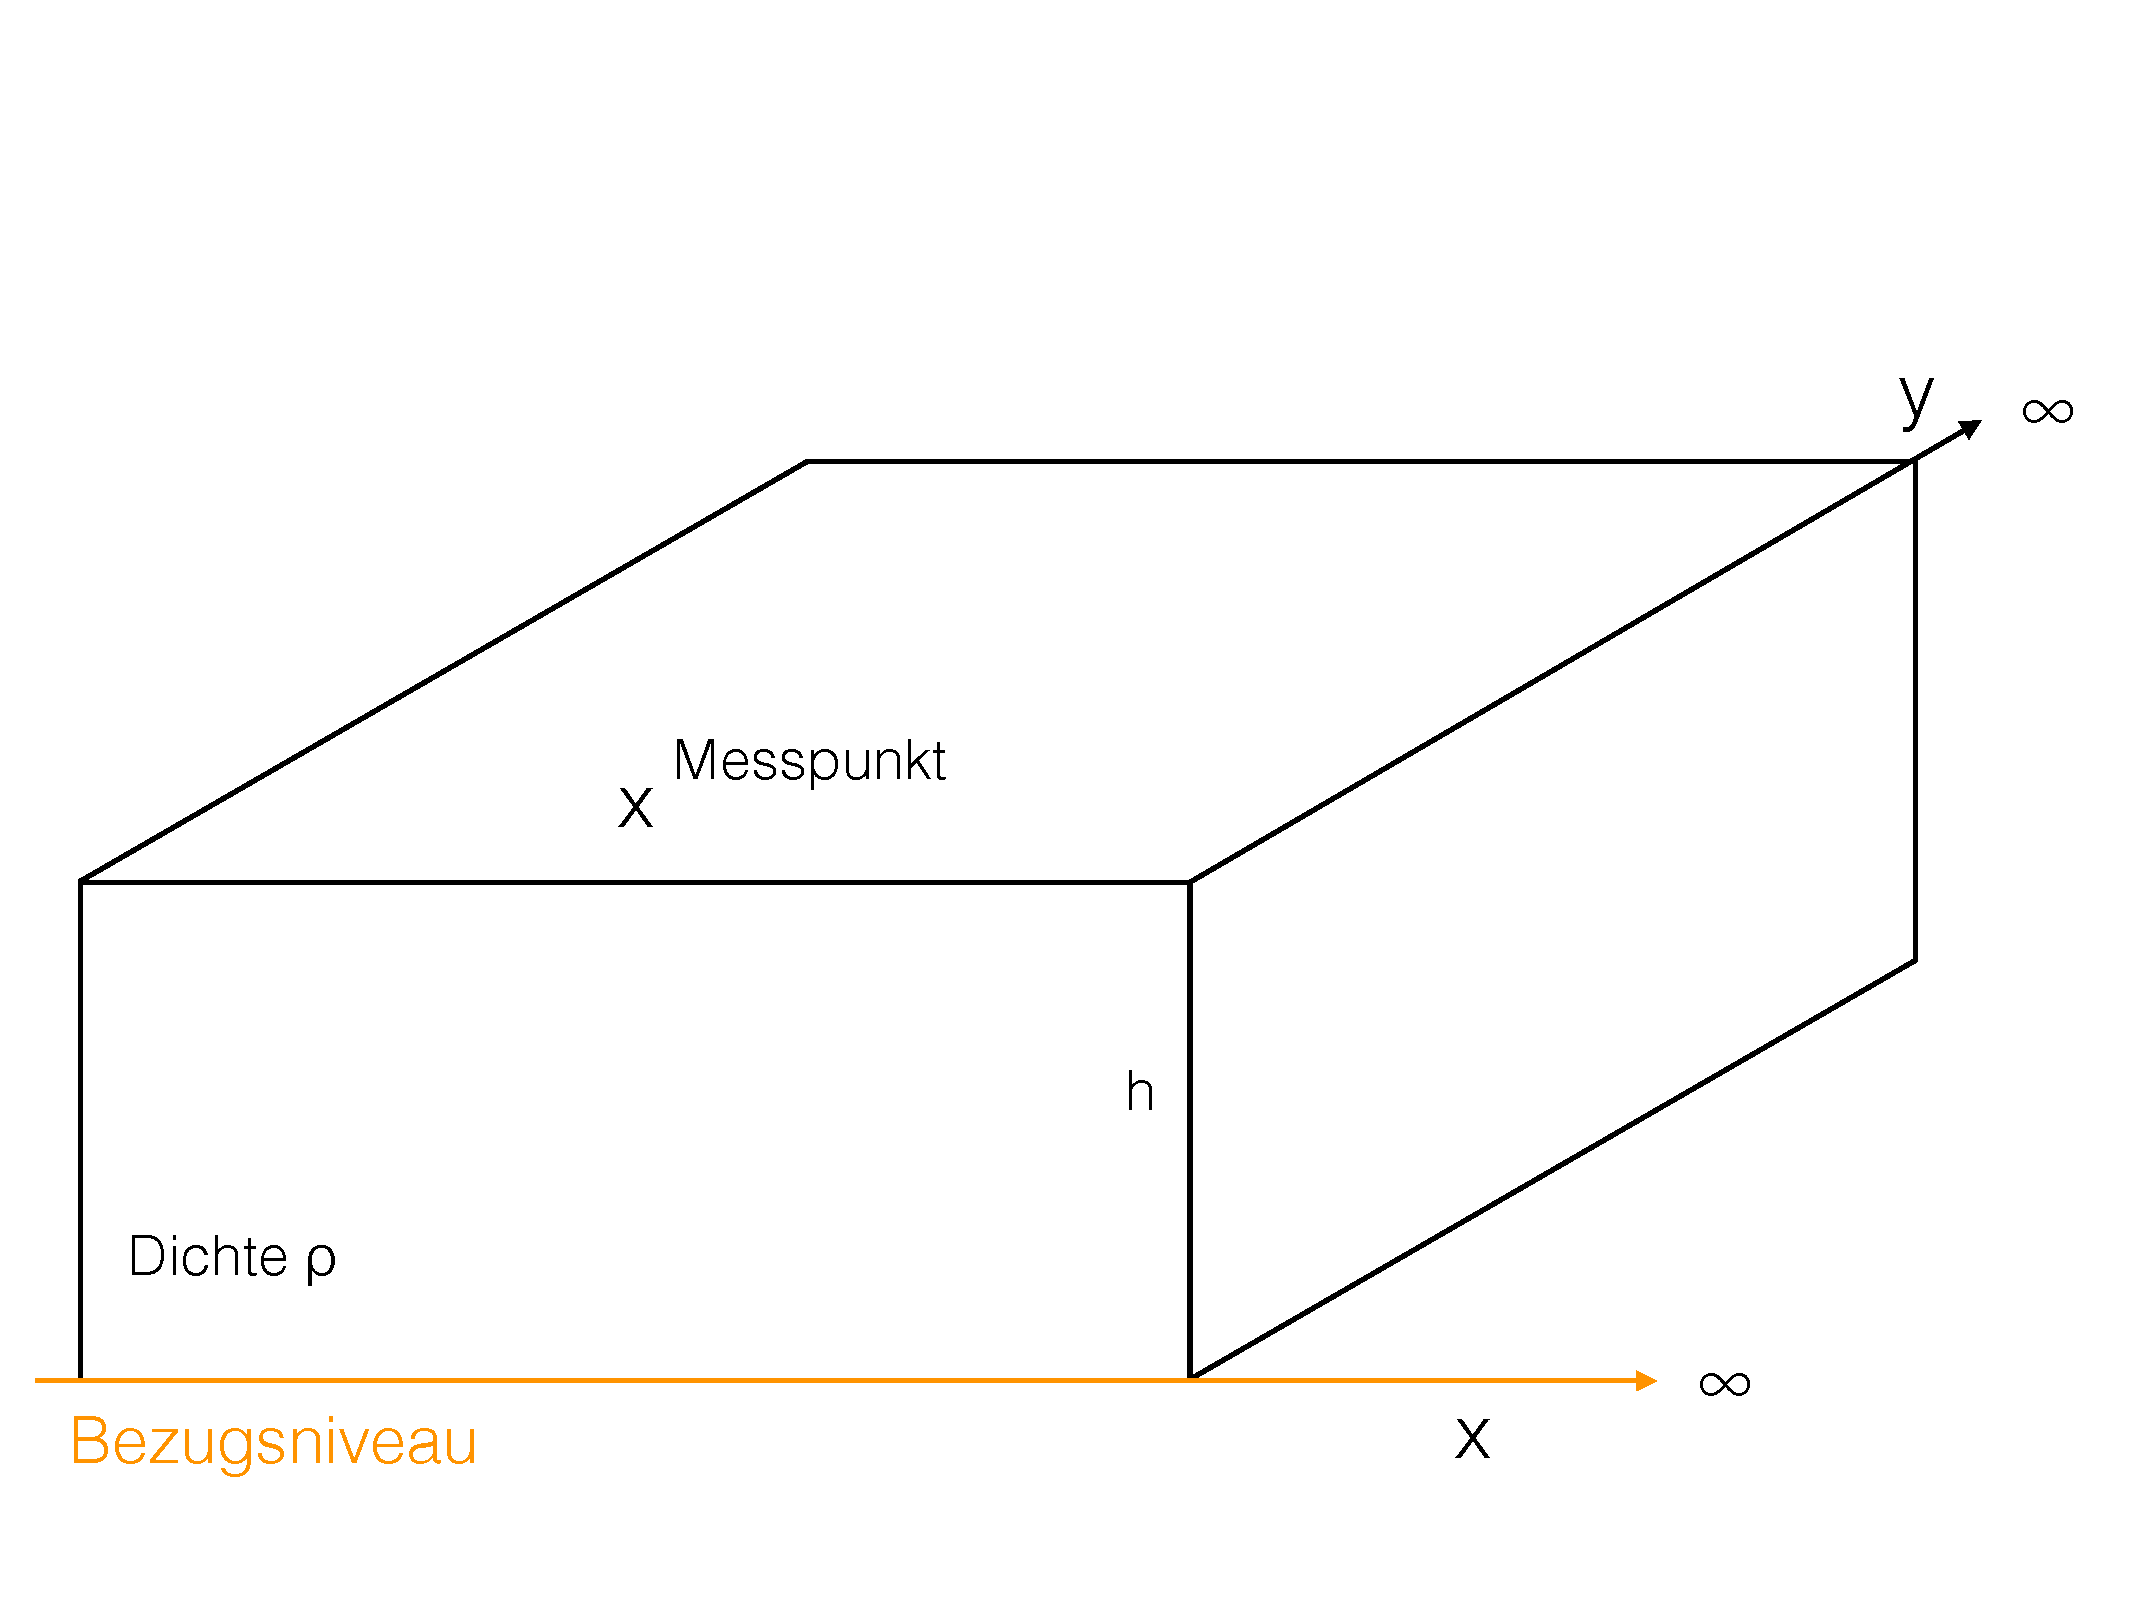
\includegraphics[width = \textwidth]{GravimetrieBilder/Bouguer-Reduktion2}
\end{figure}

Ihre Schwerewirkung berechnet sich so: \begin{equation*}
	\delta_{g_B} = 2 \pi \cdot G \cdot \rho \cdot h
\end{equation*}
Wir betrachten ein Beispiel: \begin{align*}
	&h = 10\,\si{m}, \quad \rho = 2,39\,\si{\frac{kg}{m^3}} \quad \text{(Sedimentgestein)}\\
	&\Rightarrow \delta_{g_B} = 1\,\si{m Gal}
\end{align*}

\subsubsection{Bouguer-Anomalie}
Im Gegensatz zur Freiluftanomalie rechnet man bei der Bouguer-Anomalie die Bouguer-Korrektur, also die Korrektur der Schwerewirkung der Gesteinsmasse, mit ein. Diese Berechnung spiegelt die Dichteanomalie im Untergrund gut wider. \begin{equation*}
	\Delta g_{FL} = g(x, y, z, t) - g(t) - \gamma_0 - \delta_{\gamma_0} - \delta_{g_{FL}} - \delta_{g_B}
\end{equation*} 

\subsection{Topographische Reduktion}
Bei der Bouguer-Reduktion haben wir bereits gelernt, dass Gesteinsmassen einen Einfluss auf das Messergebnis haben. Das heißt, dass wir nicht nur die Gesteinsmasse zwischen Bezugsniveau und Messpunkt, sondern auch große Gesteinsmassen in der Umgebung berücksichtigen müssen. Solche Massen sind beispielsweise hohe Berge. Auch tiefe Täler und Schluchten der Umgebung haben Einfluss. Die seitliche Schwerewirkung ist bei kleineren Bergen oder Hügeln vernachlässigbar gering, spielt aber bei Messungen in den Alpen oder im Himalaya eine wichtige Rolle und sollte daher nicht missachtet werden. \par
Um die topographische Korrektur berechnen zu können, nähert man die Berge der Umgebung als Aneinanderreihung von Zylindern an. 

\begin{figure}[H]
	\centering
	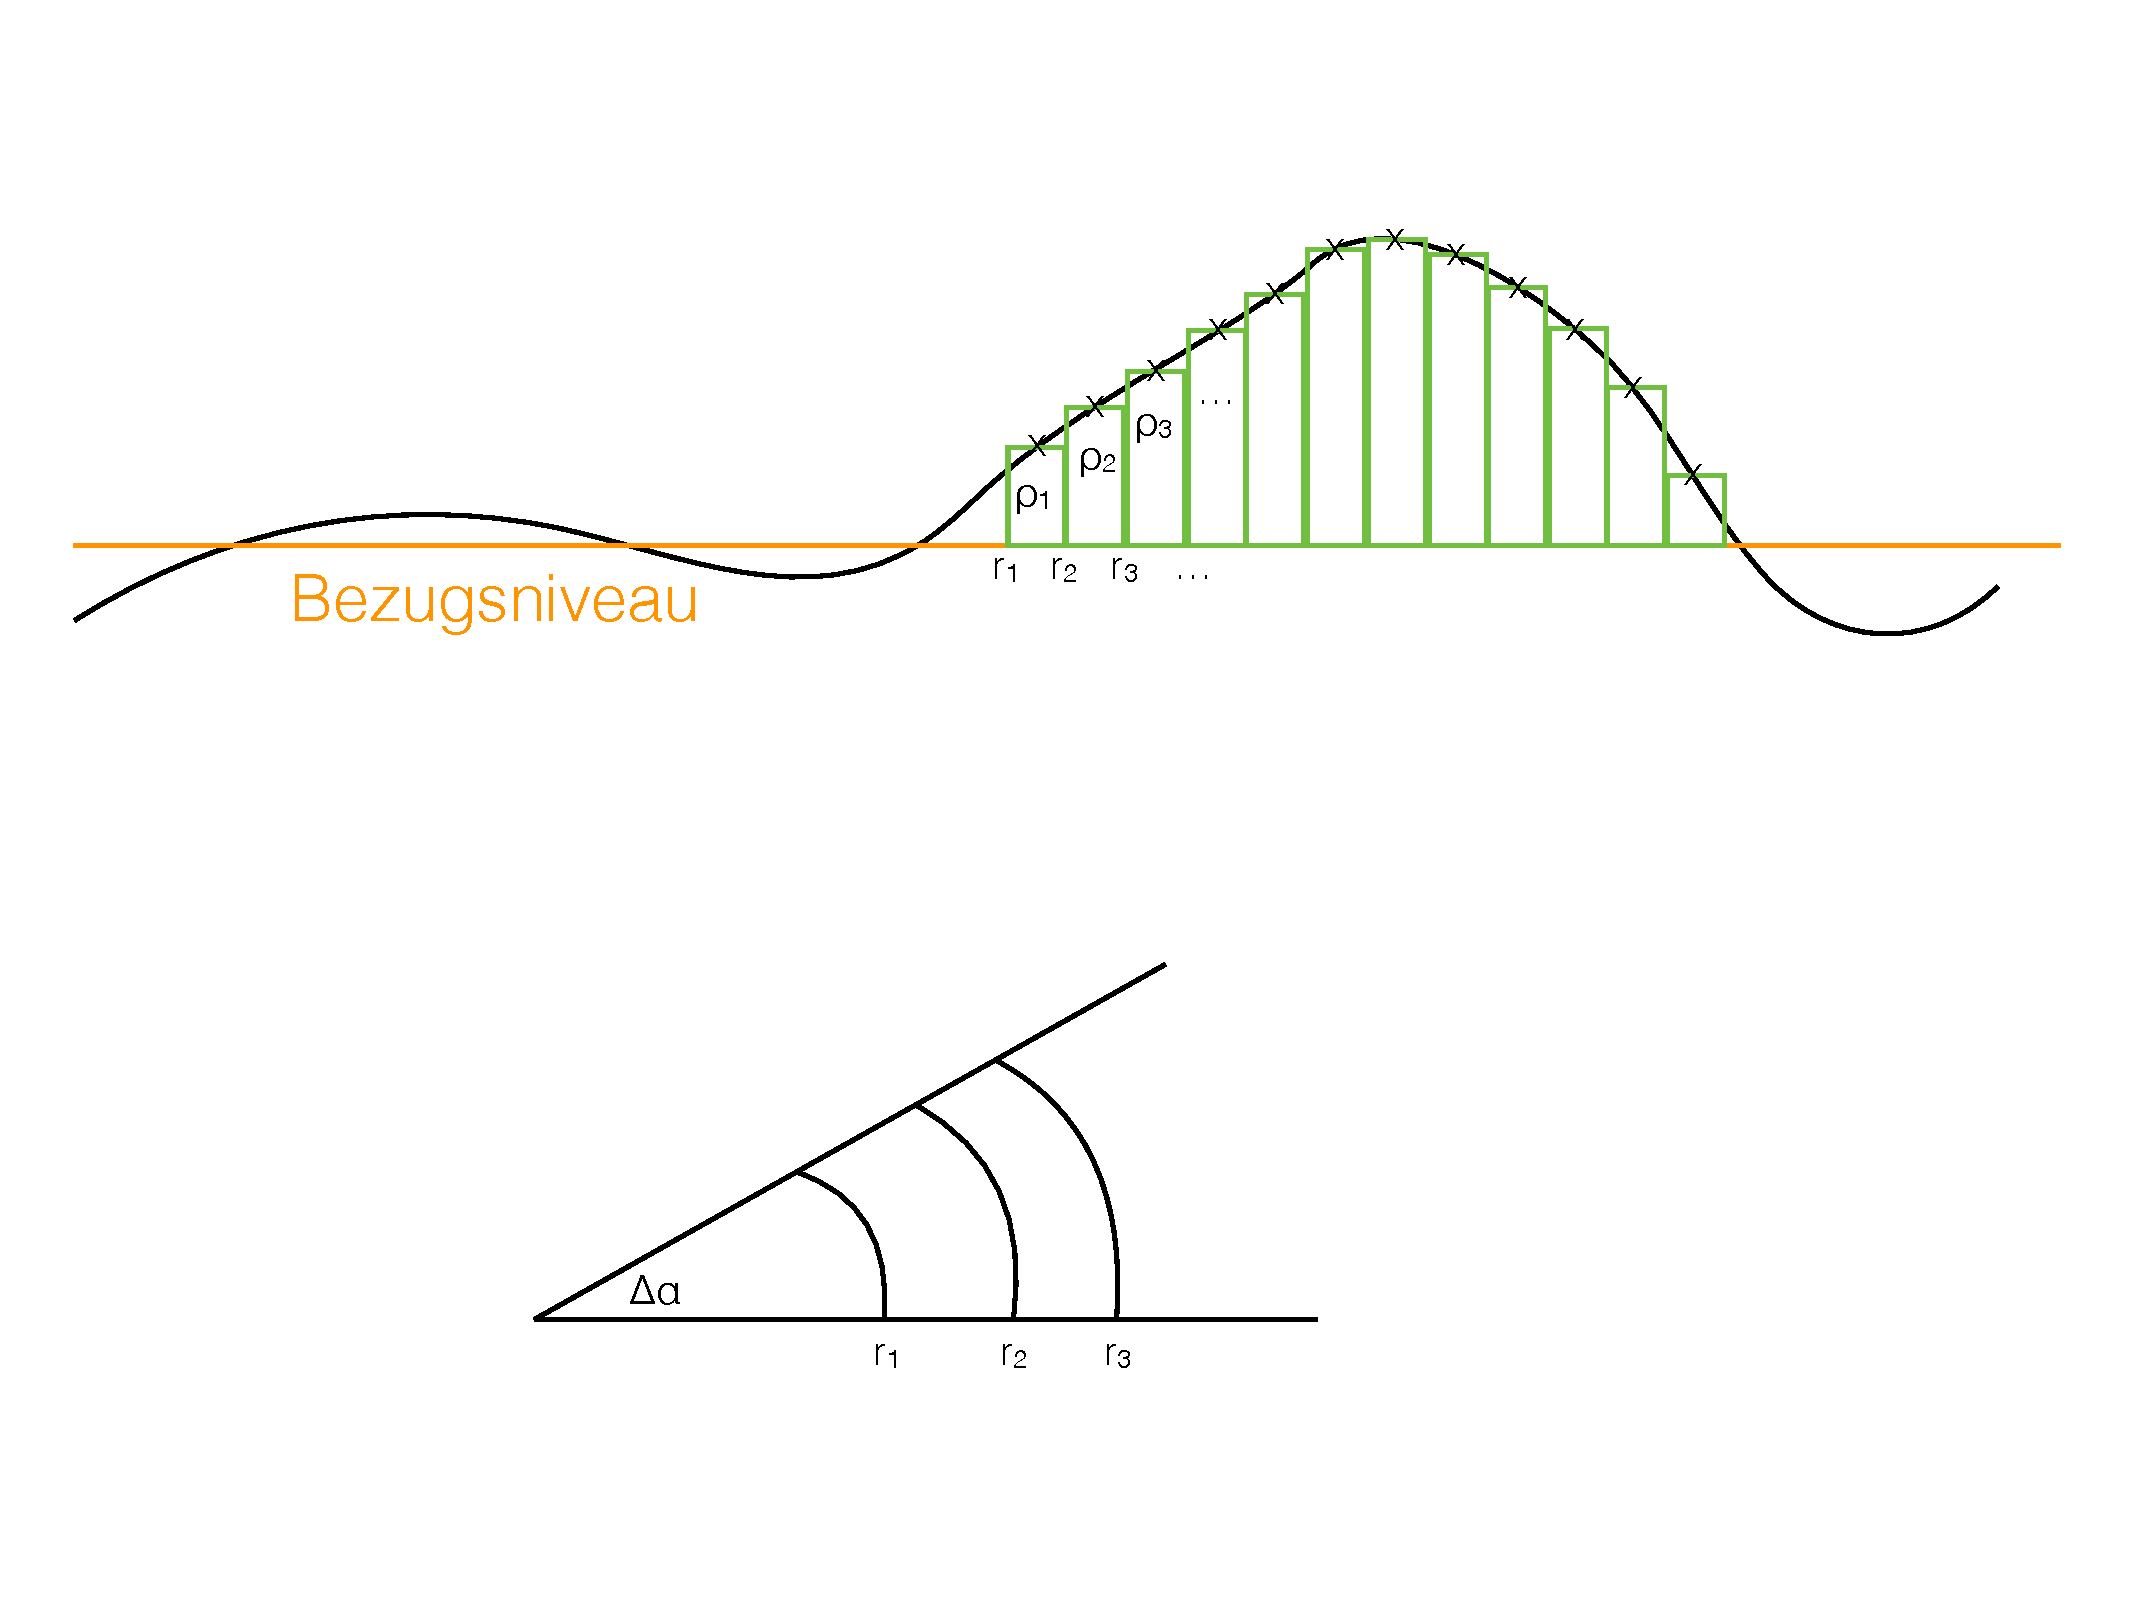
\includegraphics[width = \textwidth]{GravimetrieBilder/TopographischeReduktion}
\end{figure}

Die Summe ihrer Schwerewirkungen ergibt dann die topographische Reduktion: \begin{equation*}
	\delta_{g_{\text{Top}}} = \sum_{i} \rho_{i} \cdot \Delta \alpha \cdot \left( r_{i + 1} - r_i + \sqrt{r_i^2 + h_i^2} - \sqrt{r_{i + 1}^2 + h_i^2}  \right)
\end{equation*}

\section{Messmethodik}
Die Messgeräte, mit denen gravimetrische Messungen durchgeführt werden, nennt man Gravimeter. Im Folgenden wollen wir uns zwei Typen von Gravimetern anschauen.

\subsection{Absolutgravimeter}
Durch den Fall eines Körpers wird im Absolutgravimeter die lokale Fallbeschleunigung gemessen. Das Messergebnis ist der absolute Wert der Schwerebeschleunigung, weshalb diese Messgeräte an jedem Ort, auch außerhalb der Erde, ohne Kalibrierung eingesetzt werden können.
Eine andere Form der Absolutgravimeter vermisst die Schwere mit Hilfe einer Pendelschwingung.

\subsection{Relativgravimeter}
Ein Relativgravimeter vermisst die Veränderung der Schwerebeschleunigung bezüglich eines Nullpunkts. Im Innern dieser Gravimeter befindet sich eine Feder, die durch die Gravitationskraft gedehnt wird. Diese Dehnung wird kompensiert, und die Stärke dieser Kompensation wird gemessen. Die Feder wird aber nicht vertikal aufgehängt, da die Auslenkung der Feder bei geringer Varianz der Schwere nicht ausreichend groß ist, um exakte Messungen durchführen zu können. Die Feder wird daher so angebracht, dass eine geringe Veränderung der Schwere eine große Auslenkung der Feder zur Folge hat. Im LaCoste-Romberg-Gravimeter geschieht dies beispielsweise durch eine schräge Aufhängung der Feder. 









